\documentclass[a4paper]{article}
\usepackage[utf8]{inputenc}
\usepackage{graphicx}
\usepackage{hyperref}
\usepackage{url}
\usepackage[english]{babel}
\usepackage[super]{nth}
\usepackage{fancyhdr}
\usepackage{tabu}
\usepackage{multirow}
\usepackage{cite}
\usepackage{amsmath}
\usepackage{color}
\usepackage{subcaption}
\usepackage{titlesec}


\widowpenalties 1 10000
\raggedbottom

\newcommand{\sectionbreak}{\clearpage}

\DeclareGraphicsExtensions{.pdf,.png,.jpg,.eps}

\newcommand{\mytitle}{Zombie Apocalypse Report}
\newcommand*\mean[1]{\overline{#1}}

\newcommand{\todo}[1]{}
\renewcommand{\todo}[1]{{\color{red} TODO: {#1}}}

\pagestyle{fancy}
\fancyhf{}
\fancyhead[L]{Juraszek, Leong, Signorini, Yang}
\fancyhead[R]{\mytitle}

\fancyfoot[C]{\thepage}

\title{\mytitle}
\author{Adam Juraszek \and Ryan Leong Wei Shiong \and Matthew Signorini \and Ziying Yang}

\begin{document}
\maketitle

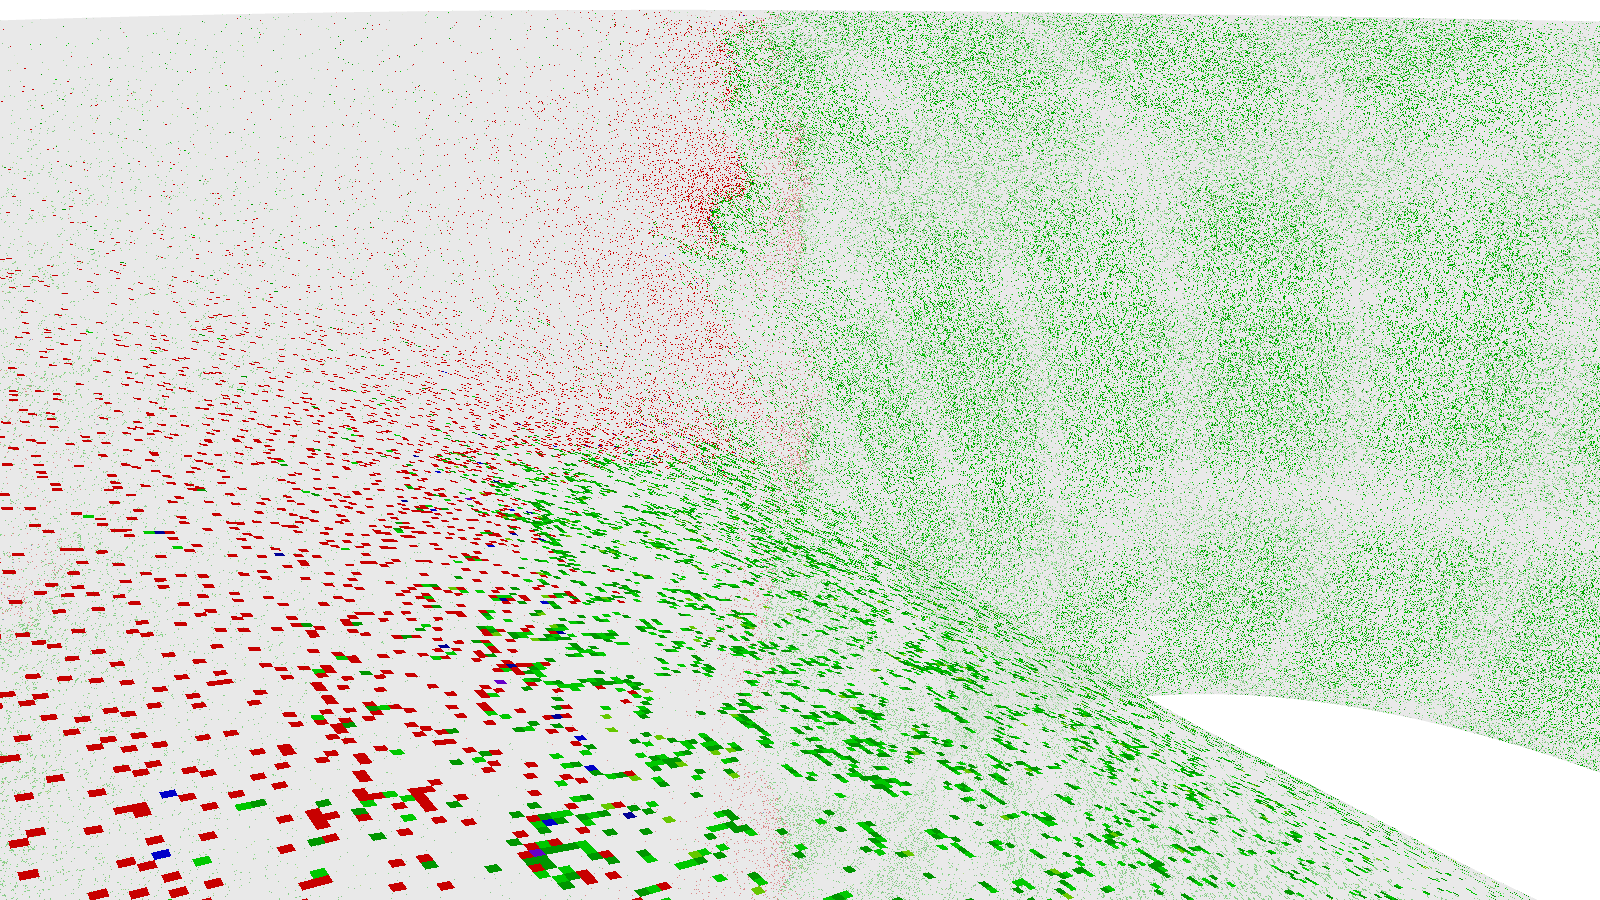
\includegraphics[width=\textwidth]{torus/title}

\newpage
\tableofcontents
\newpage

\section{Introduction}

Infectious diseases have been prevalent since the start of time.
Modelling the spread of these diseases can serve to find possible ways to stop or limit the spreading.
With the advancement of technology, computing power has increased tremendously, allowing these simulation models to be done on a greater scale.
In this project, we will implement a Zombie Infection simulation, modelling the spread of the infection on a human population.

\subsection{Zombie description}

Since this is a fictional situation, we turned to zombie references in popular culture in order to derive the characteristics of zombies.
For instance, an article on the zombies of ``World War Z'' indicates that zombies are slow moving until they sense humans around.
They will then move as fast, if not, faster than human running speed. \cite{guidetozombies}

In our model, the zombies are reanimated dead human bodies controlled by a viral infection, which is one of known types of zombies. \cite{survivingthedead}
A human becomes infected when he or she is bitten by a zombie.
The initial infection does not have any symptoms except for bite marks and short term memory loss.
The infection is latent and secretly spreads inside the body until it dominates.
The incubation period is 14 days on average, which is significantly longer than we are accustomed, however it has a medical support. \cite{mogk2011everything}
Later, during a weak moment (usually while sleeping) it causes death of the person and starts act on its own.

Zombies are strongly attracted to humans in order to infect them and humans flee from zombies.
For zombies, control of the body is poor and therefore zombie motor skills are slower and more inaccurate.
Reanimated dead bodies have only a limited durability, which we assume to be about 3 years on average\cite{zombiepedia}, and the corpse will ultimately decompose.
After this point, the zombie is no longer active or contagious.

\subsection{Requirements}

The project implementation was divided into two parts.

\begin{enumerate}
\item In the first part of this project, the task was to simulate the human and zombie population on a 500 by 500 grid.
\item We had to take into account the birth and death rate of humans, keeping them close to the current demographics of the Northern Territory in Australia.
    This hold except for the population size which is reduced to one half. \cite{project}
\item We had to model zombies which are eager to chase and infect humans.
    We had to model zombie processes starting with infection and ending with decomposition.
\item With this model, we aim to find parameters which support coexisting of both populations of humans and zombies, and also do not contradict reality.
\end{enumerate}

\subsubsection{Stability requirement}

Finding parameters that result in stable populations of both humans and zombies proved to be a challenging problem.
Since zombies decompose after a short period of time (relative to a human lifespan), it is imperative that there are regular new infection cases in order for the zombies to survive.
If there were too few humans, the zombies could not infect anybody often enough to compensate for their shorter lifespan.
On the other hand, if there are too many humans, the infection spreads very quickly, overwhelming the human population. 
This is followed by a steep decrease of both populations, typically resulting in both humans and zombies becoming extinct.
An interesting aspect of this dynamic is that zombies cannot possibly survive without humans: Zombies are not able to reproduce on their own; they depend completely on infecting humans to produce more zombies, and to replace zombies lost to decomposition. 
If the human population dies out, so too will the zombies.

\subsubsection{Environmental requirements}

The targeted run-time environment was Avoca\cite{avoca}, the IBM Blue Gene/Q\cite{bluegeneq} supercomputer.
The computer contains homogeneous 4096 nodes, each of them having 16 cores and being capable to run up to 64 threads in parallel.
A single core has rather poor performance compared to an ordinary laptop; its strength is in number of cores which can be used at the same time.

To utilise the power we had to use OpenMP\cite{openmp} -- parallelising framework built-in in common C compilers.
The first part of the project should have used a single node.
In the second part we had to add support for MPI\cite{mpi} to divide the computation into several pieces, each one of them running on one node, which is communicating with its neighbours.
The simulated world consists of a mesh of size $1000 \times 1500$, 
The goal was to run a simulation on a grid of size 1024 by 1536, corresponding to the geographical dimensions of the Northern Territory, a region in the north of Australia\cite{northernterritory}.
The simulation had to use originally 6 nodes, later it was decreased to 2 nodes.

We instead ran a simulation of infection on a small planet of size 8192 by 4096 on 128 nodes.

\section{Model}

\subsection{Infection model}

\begin{figure*}[ht]
    \centering
    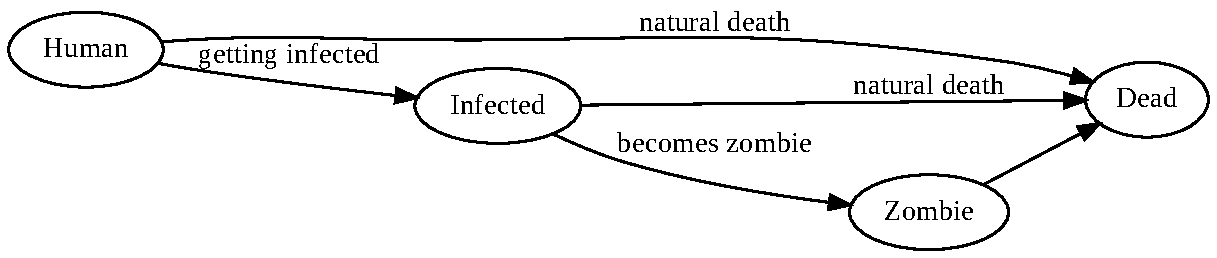
\includegraphics[width=\textwidth]{model}
    \caption{Infection model}
\end{figure*}

Our understanding is that there is no cure for the infection, and also that there is no level of immunity in the human population.
These assumptions allow us to use a simpler form of the SIR model of disease propagation, with strictly one way transitions.

In terms of the SIR model (or in this case SEIR), our model consists of four states: Humans (the susceptible group), infected humans (the exposed group), zombies (the infected group) and lastly the dead state, as there is no way for a person to recover from the infection.
An entity begins in state Human which represents a normal human being who was born, has a biological gender (either male or female), and eventually dies.
Humans become infected only by being in close proximity to a zombie.
The probability of infection is unknown but for the purpose of our model it was set to $0.75\%$ for a human within 1 kilometre of a zombie.
However small the probability seems to be, it is quite acceptable concerning the smallest time and space units being 1 day and 1 kilometre.

Humans with a latent infection, who have not developed full zombie symptoms, are in every respect normal people as far as our model is concerned, and hence can reproduce and die of a natural death.
Infected people are not contagious to the surrounding humans until they become a zombie.
Zombies are considered dead -- they are just virus-driven moving bodies; therefore we say that zombies eventually decompose instead of die.
Our model does not need to represent zombies as having a gender as they cannot reproduce nor do their properties depend on the gender of the human host.

When a human becomes infected, the length of the infection depends on the strength of the body fighting the zombie virus.
The transition happens with a certain probability that makes the average length of infection 14 days.

\subsubsection{Reproduction}

Our model provides a reasonably realistic simulation of human reproduction.
A female person can become pregnant if she is adjacent to a male person in the simulated world.
The simulation creates a child in any free cell adjacent to the mother, after a nine month gestation period has elapsed\cite{pregnancy}.
If there is no free cell available, as all adjacent cells are occupied by either people or zombies, no child is created in the simulation, and the woman is no longer pregnant.
As the zombies are of viral nature, our model assumes that an infected mother will pass on the virus to her child.
We also assume that the virus is not sexually transmitted, so there would be no virus transmission when an infected person has intercourse with a healthy human.

We have also factored in age based fertility: A female can produce children if she is between 15 and 45 years of age, and males between 15 and 80.
More than one baby can be carried in a single pregnancy -- our model supports that a female can expect up to three babies at once.
The probabilities of multiple births are in accordance with Hellin's law. \cite{hellinslaw}

\subsubsection{Age}

The model follows the Australian age distribution for both males and females.
When the simulation starts, the humans are divided into age classes based on their actual age.
Within an age class, the people are distributed uniformly.

Humans and infected are sorted into four age classes:
\begin{enumerate}
\item a child (0--15 years),
\item young (15--37.5 years),
\item middle aged (37.5--65 years),
\item elderly (65+).
\end{enumerate}

According to the latest scientific research, zombies live 3 to 5 years. \cite{zombiepedia}
Zombies are divided into two age classes:
\begin{enumerate}
\item young (0--1.5 years),
\item old (1.5+).
\end{enumerate}

Most of the properties of the entities are dependent on their gender and on age class rather than on their actual age.
The properties are:
\begin{itemize}
\item daily death rate -- the probability of a natural death per each day,
\item speed -- the probability of the entity to leave its current cell if it was its original intention.
\end{itemize}

Since the moving speed is a probability and the cell size is enormous, it only makes sense to compare the probabilities.
Females are slightly slower but still faster than zombies.
Speed of a young zombie equals to speed of an elderly human male.

Details about death probabilities are discusses later in the report.

\subsection{World representation}

The simulated world is logically one large mesh but physically it is divided into several smaller meshes.
Each mesh is processed independently on different nodes needing only synchronisation of borders at the beginning and end of each step.
Each square of this mesh is referred to as a cell, and a cell can contain at most one entity of any type; otherwise the cell is considered empty.
Two entities are said to be adjacent if they are in cells that share a border.

In the first part of the project, the world had fixed boundaries, no entity could pass through them; this is often referred as to no-flux boundary condition.
The actual size of both the logical and physical mesh was $500 \times 500$ cells.

For the second part we changed the topology from a rectangular world to a torus.
The only difference is the boundary condition, which is periodic meaning that any attempt passing through the border will be successful resulting into the entity appearing at the opposite side.
Many different sizes of logical meshes ranging from $128 \time 128$ to $16382 \times 16382$ were used for the scaling part of the report.

\begin{figure*}[ht]
    \centering
    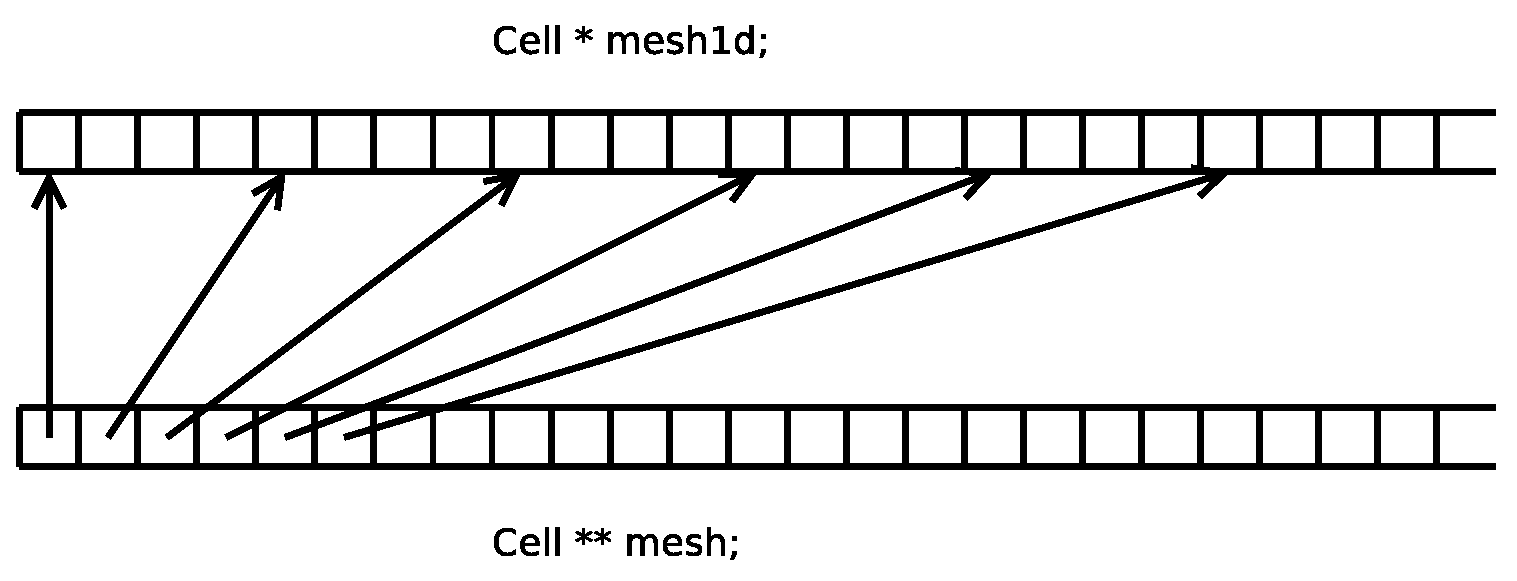
\includegraphics[width=0.8\textwidth]{mesh}
    \caption{Memory layout of the mesh}
\end{figure*}

Instead of using classic 2D array, we rather allocated huge 1D array and then created another array, whose elements point to elements of 1D array.
Not only does it allow us the same access via \verb|world->mesh[x][y]|, but also ensures that the whole mesh is a continuous chunk of memory.
This is very important because we can use \verb|MPI_Type_vector| and don't have to create extra buffers.

In order to maintain all information during the whole simulation of a time step, two worlds are used.
Input world contains all information and is never changed.
Output world is empty in the beginning and is filled by processed entities. 

\subsubsection{Mesh division}

If a simulation is running on a single node, the size of logical and physical mesh is the same.
Otherwise, when more nodes are used, the best division of the logical mesh is found.
The optimal division has these properties:
\begin{itemize}
\item the layout of physical meshes creates a grid,
\item physical meshes have the same width and height,
\item the number of meshes next to each other times the number of meshes on top of each other is equal to the total number of nodes,
\item perimeter of all meshes is the least possible.
\end{itemize}

These criteria allows an easy communication between neighbours, utilisation of all nodes and also transmitting the least possible amount of data.
As the number of nodes is small (256 or less), all possibilities can be tried; intuitively we know that square physical meshes are the optimal ones.

In order to communicate with a different node, we need to know its rank.
MPI provides a convenient way how to address the neighbour in particular direction -- the Cartesian communicators.
Each node is assigned a rank, which Cartesian communicator translates into 2 coordinates which we interpret as position of the physical mesh inside the logical mesh among other physical meshes.
The Cartesian communicator can shift a rank in any direction; values $-1$ and 1 refer to the neighbours.
It can also model a periodic situation, for example left neighbour of the leftmost node is the rightmost one and vice versa.

If the program is compiled with MPI support, the Cartesian communicator is always used, even if the world runs on a single node, in which case all neighbours are the node itself.

When the simulation starts, people and zombies are randomly distributed in the world.
Having several world parts requires extra caution.
The total number of people is divided among the parts based on area fraction.
The world also starts with two zombies near to each other \cite{project}.
We simply place all (both) zombies into the same world part.

\subsubsection{Movement}

\begin{figure*}[ht]
    \centering
    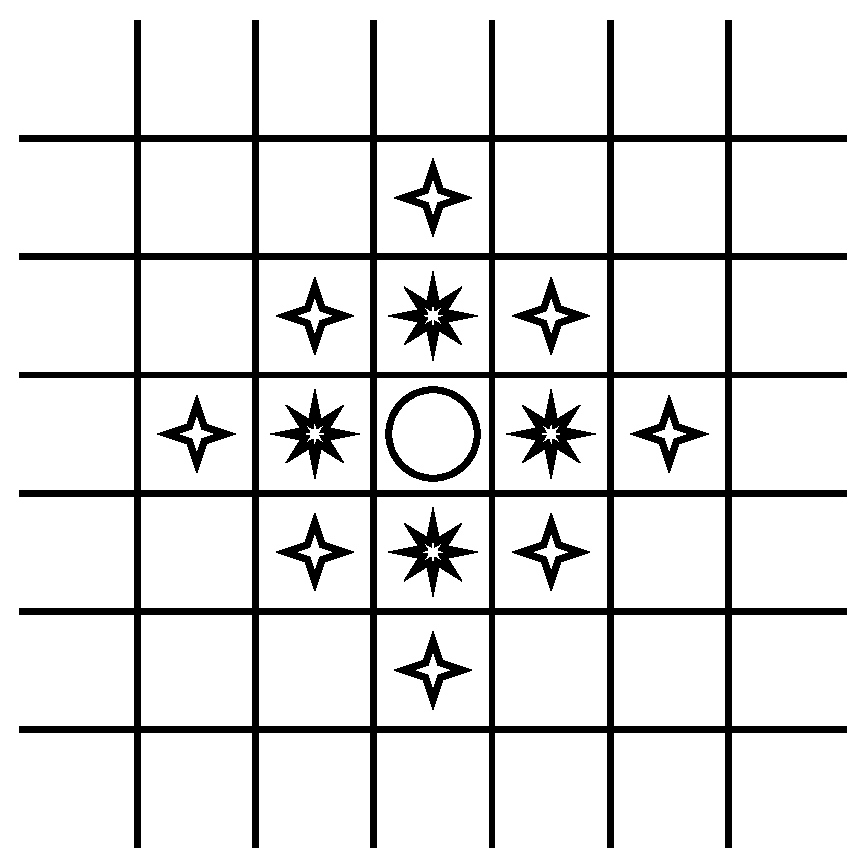
\includegraphics[width=0.3\textwidth]{movement}
    \caption{Considered cells when planning movement}
\end{figure*}

\begin{figure*}[ht]
    \centering
    \begin{tabu} {| X[1.8,c,p] || X[1,c,p] | X[1,c,p] | X[1,c,p] | X[1,c,p] | X[1.2,c,p] |}
        \rowfont{\bfseries}
        \hline
        sees &
        Wall\footnotemark &
        Empty tile&
        Zombie &
        Same gender &
        Opposite gender \\
        \hline
        \hline
        \textbf{Living entity} & -- & + & -- & + & ++ \\
        \hline
        \textbf{Zombie} & -- & + & + & \multicolumn{2}{c|}{ ++ } \\
        \hline
    \end{tabu}
    \caption{Affinity to directed situations for each type}
\end{figure*}

All entities, including zombies, share the same movement planning model.
They differ mainly in preference where to go.

Each entity determines its optimal direction based on surrounding 12 cells as shown on the diagram.
The cells to which it can get within one move are marked with a fancy star; cells accessible within two moves are marked with a simple star.
When considering directions, the adjacent cells always have higher priority.

Each entity rates each of these cells based on their content.
The preference for direction is then calculated as a weighted sum of complex numbers corresponding to particular directions.
The values of preference were chosen to mimic expected behaviour.
Better results could be achieved by a more sophisticated (genetic) algorithm or by a more thorough analysis.
The current estimates can be seen in the table below.
To the current preferred direction the potential direction of the last move is added, that simulates inertia of movement and as a result it makes the movement targeted.

% this adds footnote for the Wall which is in the table. Make sure it is on the same page!
\footnotetext{Wall was used only the first part of the project with no-flux boundary condition.}

After the optimal weighted direction is calculated, it is translated to a particular direction, or stay instruction if the absolute value is not sufficient.
The direction may randomly change clock-wise or counter-clock-wise simulating evading obstacles, which are not modelled in the world.
Then the cell in the resulting direction is tested whether it is free; if it is not, the clock-wise or counter-clock-wise one is chosen.
In the worst case, the entity stays at its current tile.
The entity moves only if its speed (expressed as probability) is sufficient.

\subsubsection{Borders}

Each physical mesh has a border 2 cells wide; this border has multiple purposes and is used differently in certain parts of the application.

If the movement of an entity at the end of the world is being processed, it would be necessary to make sure all the time that the nearby cell is still in the world.
Extending the world by the border simplifies the processing, no tests are necessary.

\begin{figure*}[ht]
    \begin{subfigure}[b]{.5\linewidth}
        \centering
        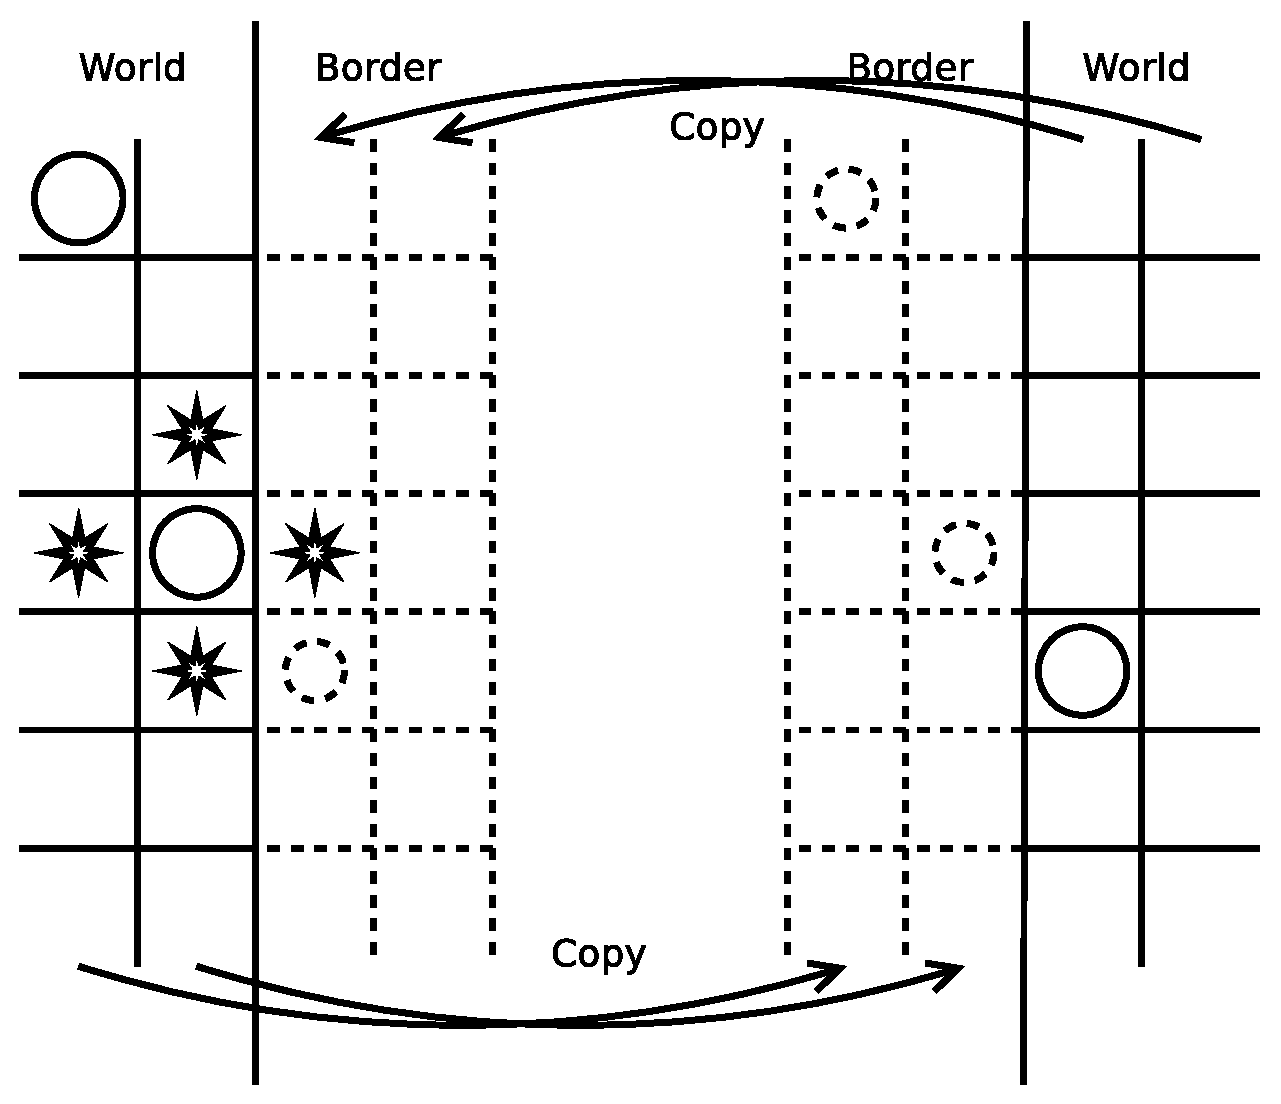
\includegraphics[width=0.9\textwidth]{border1}
        \caption{Borders of the input world}
        \end{subfigure}%
    \begin{subfigure}[b]{.5\linewidth}
        \centering
        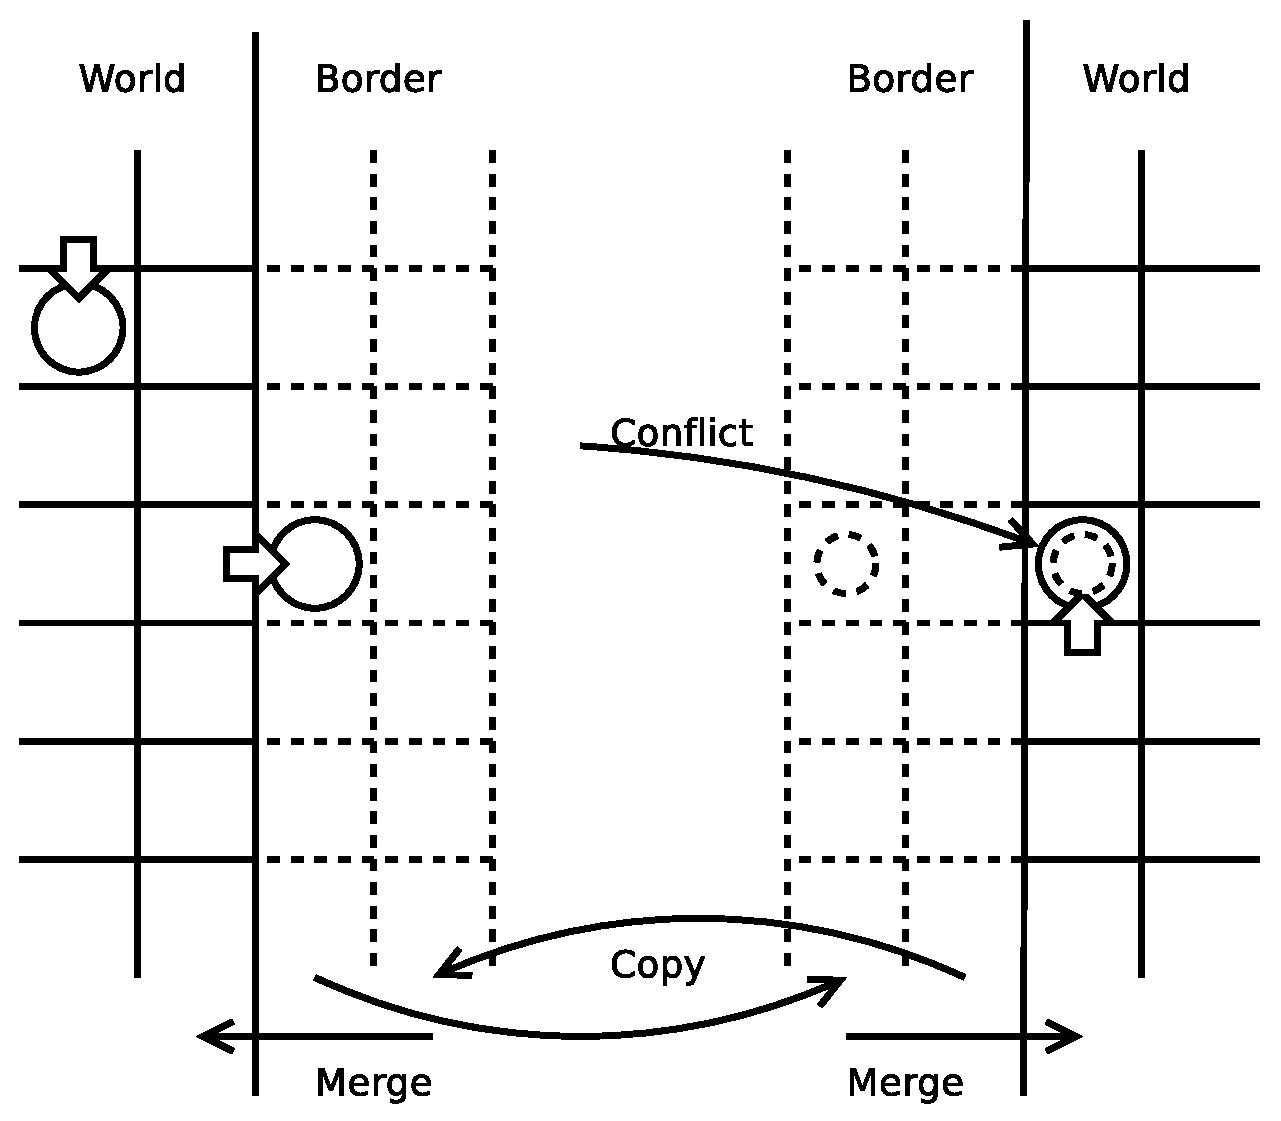
\includegraphics[width=0.9\textwidth]{border2}
        \caption{Borders of the output world}
    \end{subfigure}
\end{figure*}

Another issue which the border solves is with movement planning.
With periodic boundary condition, an entity needs to see what entities are in the last rows/column of an adjacent cell.
We cannot afford to ask the adjacent world all the time.
That is the reason why all the data are copied prior to each simulation step.
For example the two rightmost columns are copied to the left border of the world part which is logically to the right.
There are no conflicts; the data which were in the border are insignificant.

Similar argument applies to a situation when an entity leaves the current world part and should be moved to the adjacent one.
The moving entities are left in the border until the simulation of the current step ends and then they all are transferred.
The entities can move only one cell at a time and therefore we only need to copy one row/column, not both of them.
However, we cannot copy the rows/columns blindly, they would overwrite existing entities.
Luckily, we have one row/column free, the outer one of the border as no entities may get there.
We use it as a buffer; after all borders are transferred, we merge it to the last row/column of the world.
In this case, conflicts may happen as it is shown in the figure.

\subsubsection{Simulation}

\begin{figure*}[ht]
    \centering
\begin{verbatim}
void simulateStep(WorldPtr input, WorldPtr output) {
    output->clock = input->clock + 1;

    sendRecieveBorder(input);
    // while waiting for input border
    simulateStep1(input, output);
    sendRecieveBorderFinish(input);

    // this needs input with border
    simulateStep2(input, output);

    sendReceiveGhosts(output);
    // while waiting for ghost cell movement
    resetWorld(input);
    sendReceiveGhostsFinish(output);
}
\end{verbatim}
    \caption{Source code of the simulation}
\end{figure*}

Some of the natural processes do not need to access adjacent cells, we refer to them as local.
They are:
\begin{itemize}
\item death of a human or an infected,
\item decomposition of a zombie,
\item transition of an infected to a zombie.
\end{itemize}

In the beginning of the simulation step we also need to send and receive parts of borders of the input world.
These two tasks can be run in parallel.
While the data are being send and received (asynchronously), local processes are handled.
After that there is still some time spend by waiting (see the result section).

The rest of the processes needs neighbour cells:
\begin{itemize}
\item transition of a human into an infected,
\item giving birth to children,
\item couple making love,
\item movement.
\end{itemize}

Similar concept applies to sending sends and receives of parts of borders of output worlds when the simulation is finished.
We can run that in parallel with world cleaning.

\subsection{Initialisation of the population}

\subsubsection{Age structure and death rate}

\begin{figure*}[ht]
    \centering
    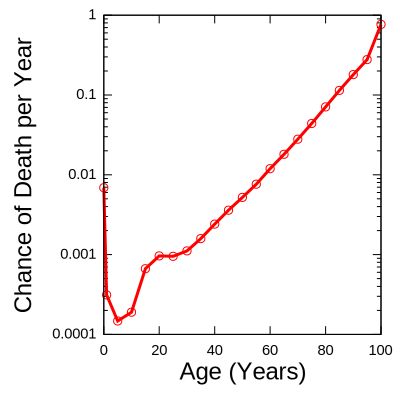
\includegraphics[width=0.6\textwidth]{USGompertzCurve}
    \caption{Mortality rates for US in 2003}
\end{figure*}

According to the Australian age structure\cite{agestructure} and median of age 37.3 years \cite{demographicsaustralia}, initialised humans are divided into four age classes.
Based on mortality rates graph for US in 2003 (shown in the figure) and Gompertz–Makeham law \cite{mortalitylaw} the average probabilities of a human dying in these four age stages are approximately related as 
$$ \mean{P(\text{Elder Death})} = 10\: \mean{P(\text{Middle Age Death})} $$
$$ = 80\: \mean{P(\text{Young Death})} = 160\: \mean{P(\text{Child Death})} $$

We worked out the probability of a person dying on any given day based on data from the Australian Bureau of Statistics on the number of people who died in 2012\cite{absdeath}:
$$ \mean{P(\text{Australia Death})} = \frac{\text{people who died (in 2012)}}{\text{population size (in 2012)}} $$
$$ = \frac{147098}{23319400} = 0.63\%/\text{year} = 0.0017\%/\text{day} $$

The death rates for each age class can be calculated and expresses as shown in the table below.

\begin{figure*}[ht]
    \centering
    \begin{tabu} {| X[1.1,c,p] || X[0.7,c,p] | X[1.2,c,p] | X[1.1,c,p] | X[1,c,p] |}
        \rowfont{\bfseries}
        \hline
        Class Name &
        Age Range &
        Distribution &
        Average Death Rate (per day) &
        Death Rate (per day) \\
        \hline
        \hline
        \textbf{Child} & 0--15 & 18.2\% & \multirow{4}{*}{0.0017\%} & 0.00006\% \\
        \cline{1-3}\cline{5-5}
        \textbf{Young} & 15--37.5 & 31.8\% & & 0.00012\% \\
        \cline{1-3}\cline{5-5}
        \textbf{Middle Age} & 37.5--65 & 35.6\% & & 0.00096\% \\
        \cline{1-3}\cline{5-5}
        \textbf{Elderly} & 65+ & 14.4\% & & 0.0096\% \\
        \hline
    \end{tabu}
    \caption{Death rate of age classes}
\end{figure*}

It is well known fact that females live longer than males.
We incorporated it as a difference of death probabilities, which is equal to
$$ \text{ratio} = \frac{\text{Female lifespan}}{\text{Male lifespan}} = \frac{\text{Probability of Male Death}}{\text{Probability of Female Death}} = \frac{82.4}{78.5} = 1.05 $$
Males' probabilities are multiplied by square root of this ratio and females' are divided.

\subsubsection{Birth rate}

There are two situations when the birth rate is used in a way.

First, when the simulation starts, some females should be pregnant.
The estimated probability of a female in fertility period being pregnant is:
$$ P(\text{Pregnant Female in Fertility Period}) $$
$$ = \frac{\text{average number of children per female life} \times \text{pregnancy duration}}{\text{average length of fertility period}} $$
$$ = \frac{1.77 \times 9 (\text{months})}{30 (\text{years})} = 4.36\% $$

Although we had access to birth rates, we did not try to utilise them during the simulation because of the excessive difficulty of calculations.
Simple approach of counting probabilities of a male-female couples on a mesh do not work when the movement is targeted (as discussed earlier).
We also model fertilisation and pregnancy periods which naturally limit the baby procreation.

In order to determine the appropriate birth rate, we ran the simulation for several generations without any zombies, and by trial and error found the right rate that ensured that the human population size was stable or slightly increasing.
In this way we determined a probability of child being conceived each time a couple makes love equal to 0.00073, which is a number that does not make sense without context of the implemented model.
This is just a small price for much more realistic model of child birth.

\subsubsection{Sex ratio}

The birth ratio between males and females is 1.06. \cite{cia}
Hence the ratio of male to female children is initialised as
$$ \text{Male Child} : \text{Female Child} = 0.5146 : 0.4854 $$

However, the ratio is different when the simulation starts.
The ratio in Australia is currently 1.01 and can be expressed as \cite{cia}
$$ \text{Male} : \text{Female} = 0.5025 : 0.4975 $$

\subsubsection{Population Density}

For the purpose of the first part of the project, we used the density of the Northern Territory, which was$0.17\text{people}/\text{km}^2$  prior to the zombie apocalypse. \cite{northernterritory}
When the viral infection starts, the authorities estimate that approximately half of the population will move from Australia to Sweden. \cite{project}
Since the simulated mesh was $500 \times 500$, the initial number of simulated humans was
$$ 500 \cdot 500 \cdot \frac{0.17}{2} = 21250 $$

In the second part, even though we abandoned the Northern Territory, we did not change the density because it is one of the parameters which the stability of the model is highly dependent on.

\section{Population stability}

In the first part of the project, the most crucial task was to make both populations stable.
Here we present our attempts and the final results.
Values in this section relate only to the first part of the project; the second part used different boundary condition which makes a big difference.

\subsection{Population size}

Making the model stable without zombies was easy.
In order to add zombies we had to change the model a bit to deal with zombies and their dynamic population size.

\begin{figure*}[pht]
    \centering
    \includegraphics[width=\textwidth]{uncontrolled_birth}
    \caption{Uncontrolled birth}
\end{figure*}

The natural choice to change was the birth rate, which was first set to be constant.
As there are less humans, the constant birth rate, which works for original population, cannot be used any more.
Humans do not meet as often and therefore their likelihood of making love decrease and their population will as well.
The higher the initial population the more zombies will be created, and the sooner the model will collapse.
After about only 74 years, zombies died out and human population dropped to 940 individuals; humans eventually die out.

\begin{figure*}[pht]
    \centering
    \includegraphics[width=\textwidth]{equal_birth}
    \caption{Equal birth}
\end{figure*}

Then we tried to compensate the deaths (both natural and humans becoming zombies) by producing the same number of children.
This should have kept the population stable at any population size.
We hoped that after the initial drop, the population would become stable at a lower number of humans and zombies.
Unfortunately, it did not work as expected; it was even worse than the uncontrolled one.
The zombies died out after 72 years with 578 humans left alive (not for long).

\begin{figure*}[pht]
    \centering
    \includegraphics[width=\textwidth]{density_birth}
    \caption{Density dependent birth}
\end{figure*}

The next attempt used the initial birth rate multiplied by a quotient which was defined as a ratio of initial and current population.
As the population drops down, the humans shall reproduce more often and therefore raise back to the original population size.
The model without zombies using this technique is much more stable, however the quotient is not strong enough to deal with zombies.
A populations sizes during the simulation are shown in the figure.
Zombies still died out after 82 years with 2170 humans alive, however this time the human population could recover and get close to the initial size in two centuries.

\subsubsection{Function of densities ratio}

\begin{figure*}[pht]
    \centering
    \includegraphics[width=\textwidth]{fertilisation_probability}
    \caption{Density dependent fertilisation functions}
\end{figure*}

\begin{figure*}[pht]
    \centering
    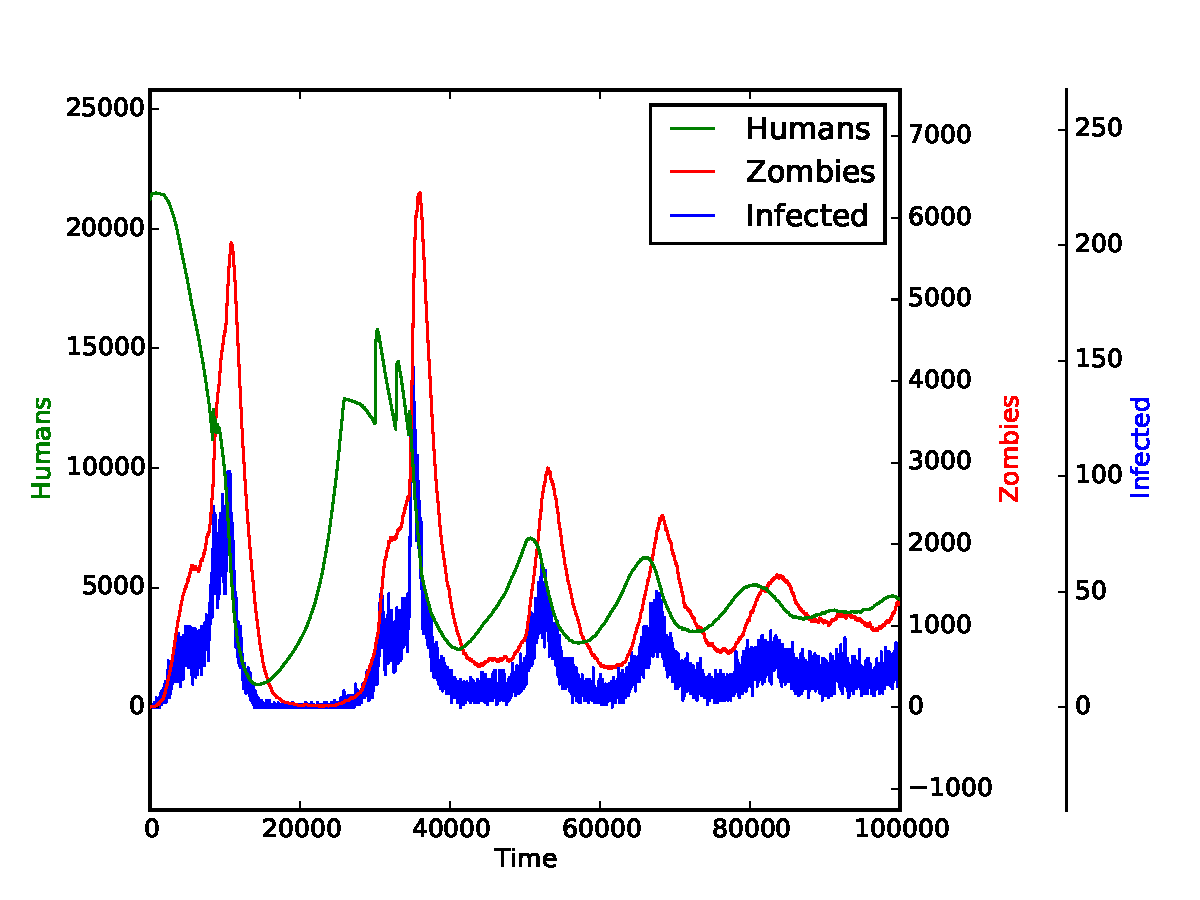
\includegraphics[width=\textwidth]{stable}
    \caption{Stable populations of humans and zombies}
\end{figure*}

The aim of the birth rate function, which depends on population density, is to allow free initial decrease of humans, and then ``kick-in'' when the population is lower.
The initial stage is important because otherwise the population of zombies would become too high and the model would not be stable.
We tried to use several function which has the mentioned properties and also become identity close to initial density.
Our candidate for the quotient function was $r^{r \cdot const}$, where $r$ is the ratio of population densities.
We also tried a simpler function $r^{const}$, which provided similar results.

The optimal value for the constant in exponent, let's call it situation awareness, is 2.5.
Higher values make the populations oscillate in time, and lower values makes the population unnaturally stable.
The population sizes for the full initial human population of 21,250 is shown in the figure.

\begin{figure*}[pht]
    \centering
    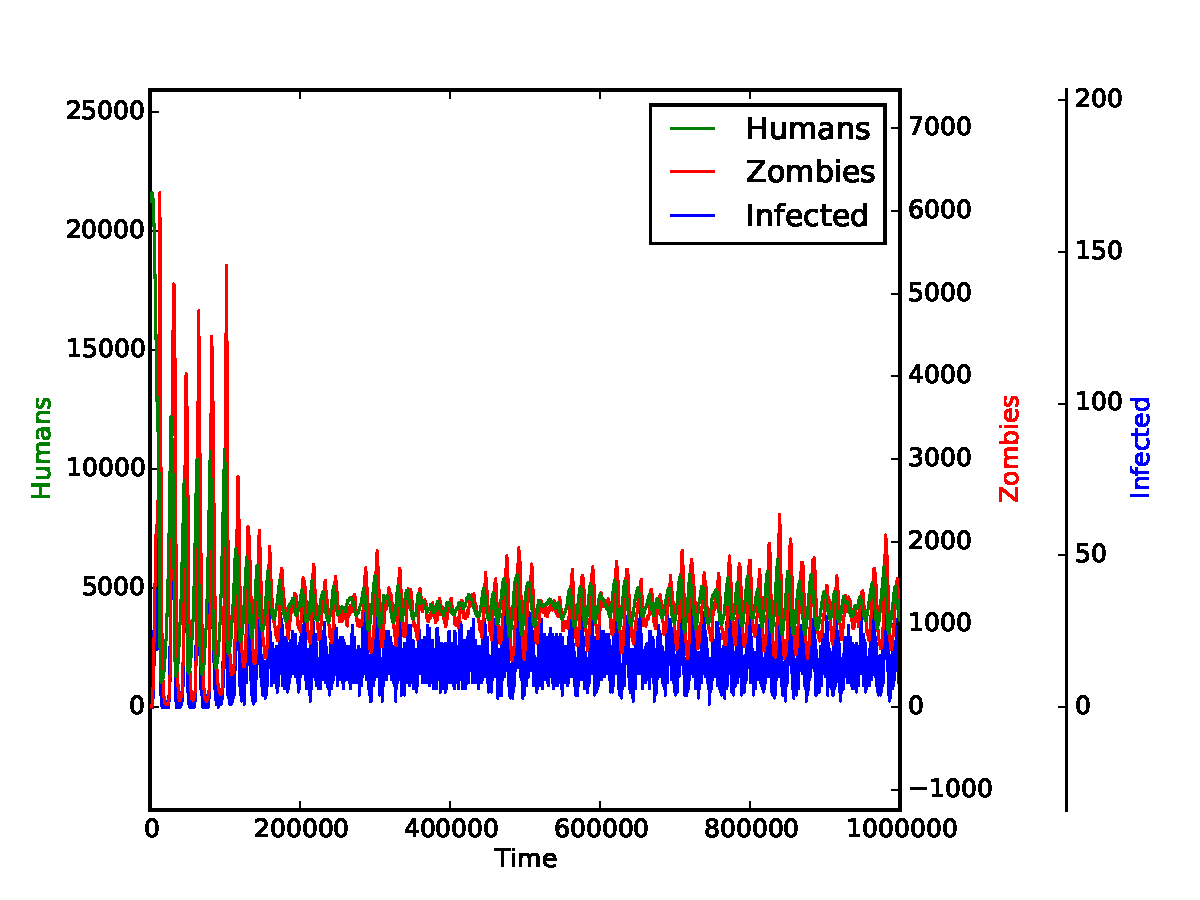
\includegraphics[width=\textwidth]{stable_1000000}
    \caption{2740 years long stable simulation}
\end{figure*}

We have also run the simulation for a longer period to discover its other properties.
As another figure of ten times longer simulation shows, the sizes of populations of human, infected and zombie make 60 years long cycles.
When the simulation starts, the swings of population sizes are becoming smaller and they eventually become constant, nonzero with occasional deflections.
To this quite stable stage the model gets after two cycles.

\subsection{Demographics}

\begin{itemize}
\item When the simulation starts, the number of demographics is exactly as described earlier.
    There are noticeable four horizontal areas which correspond to age classes.
\item After 10 years, there demographic situation remains the same, only shifted to the right.
    Zombies start to appear and their age distribution starts to spread.
\item After 50 years, after the first zombie peak, which is noticeable by the low number of young zombies and few infected, the demographic distribution has changed.
    According to model, more females are born, however being slower (and having lower daily death probability), their number becomes less than number of males.
\item After 150 years, the populations have stabilised, there are many infected and the population distributions got their final shape.
    This figure is also an example of pregnant infected female.
\item The situation at the end of the simulation after 100,000 days (approximately 274 years) is no different from the previous situation.
\end{itemize}

\begin{figure*}[pht]
    \centering
    \includegraphics[width=0.8\textwidth]{step-000000.png}
    \caption{Simulation mesh at the beginning}
    \includegraphics[width=\textwidth]{step-000000.pdf}
    \caption{Demographics at the beginning}
\end{figure*}

\begin{figure*}[pht]
    \centering
    \includegraphics[width=0.8\textwidth]{step-003650.png}
    \caption{Simulation mesh after 10 years}
    \includegraphics[width=\textwidth]{step-003650.pdf}
    \caption{Demographics after 10 years}
\end{figure*}

\begin{figure*}[pht]
    \centering
    \includegraphics[width=0.8\textwidth]{step-018250.png}
    \caption{Simulation mesh after 50 years}
    \includegraphics[width=\textwidth]{step-018250.pdf}
    \caption{Demographics after 50 years}
\end{figure*}

\begin{figure*}[pht]
    \centering
    \includegraphics[width=0.8\textwidth]{step-053100.png}
    \caption{Simulation mesh after 150 years}
    \includegraphics[width=\textwidth]{step-053100.pdf}
    \caption{Demographics after 150 years}
\end{figure*}

\begin{figure*}[pht]
    \centering
    \includegraphics[width=0.8\textwidth]{step-100000.png}
    \caption{Simulation mesh after 274 years}
    \includegraphics[width=\textwidth]{step-100000.pdf}
    \caption{Demographics after 274 years}
\end{figure*}

\subsection{Scaling}

\begin{figure*}[ht]
    \centering
    \begin{tabu} {| X[0.8,c,p] || X[1,c,p] | X[1,c,p] | X[1,c,p] |}
        \rowfont{\bfseries}
        \hline
        Threads &
        First attempt &
        Second attempt&
        Third attempt \\
        \hline
        \hline
        \textbf{1} & 180588.734000 & 180633.477000 & 180441.396000 \\
        \hline
        \textbf{2} & 94541.958000 & 95547.356000 & 94704.053000 \\
        \hline
        \textbf{4} & 49689.704000 & 50052.682000 & 50359.165000 \\
        \hline
        \textbf{8} & 25863.988000 & 26373.077000 & 26276.703000 \\
        \hline
        \textbf{16} & 14365.825000 & 14386.286000 & 14363.556000 \\
        \hline
        \textbf{32} & 10598.242000 & 10936.435000 & 10854.121000 \\
        \hline
        \textbf{64} & 14785.381000 & 14363.065000 & 14936.496000 \\
        \hline
    \end{tabu}
    \caption{Scaling depending on number of threads}
\end{figure*}

We also performed basic scaling tests which are briefly summarised in the table (running times are in milliseconds).
We ran the model three times for 1000 iterations in order to ensure the influence of randomness does not make the results odd.
We expected a perfect scaling up to 16 threads -- each of them will be assigned to a dedicated core.
Running with 32 cores still provides an improvement, but not a significant one.
The drop of performance when running with 64 threads is caused by too small size of the world.
We discuss this issue in the next section in more detail.

\section{Larger results}

In the second part of the project, we performed more scaling tests and in the end also a final simulation of a small planet.

\subsection{Scaling}

There are two types of scaling which are relevant to our project.
Firstly, strong scaling refers to how the overall running time (the wall time) varies with the number of threads used.
The second type, weak scaling, describes how the running time varies for a constant size world.

To measure the scalability of our project, we ran our simulation for a range of different world sizes, from $128 \times 128$ up to $16384 \times 16384$, and also thread counts ranging from 1 thread up to 64 threads.
The simulation was run on a single node of the Avoca cluster, with OpenMP being used for multithreading, however MPI was not used for these simulation runs since they were not run across multiple nodes.
The time taken for each simulation run was recorded in a text file, along with the number of threads and the world size for each run.
This text file was then loaded into GNU Octave for analysis.

\subsubsection{Strong scaling on 1 node}

Strong scaling is the simpler of our two metrics, and we visualised it by simply collecting all the run times for a given world size, and plotting the number of threads versus the run time in a bar graph.
We also overlayed a bar graph of the number of threads versus the run-time multiplied by the number of threads used, which is approximately the total amount of time spent by all of the threads.
In the ideal case, with perfect strong scaling, we would expect that the work would be constant regardless of whether one thread was used or 64, however our plots show that the work increases with the number of threads.
This reflects the fact that our simulation does not have perfect scaling: in terms of Amdahl's law, there is a certain fraction of the program that cannot be done in parallel, and this non parallelisable part is responsible for the growth in the work as the number of threads increases.

\begin{figure}
    \centering
    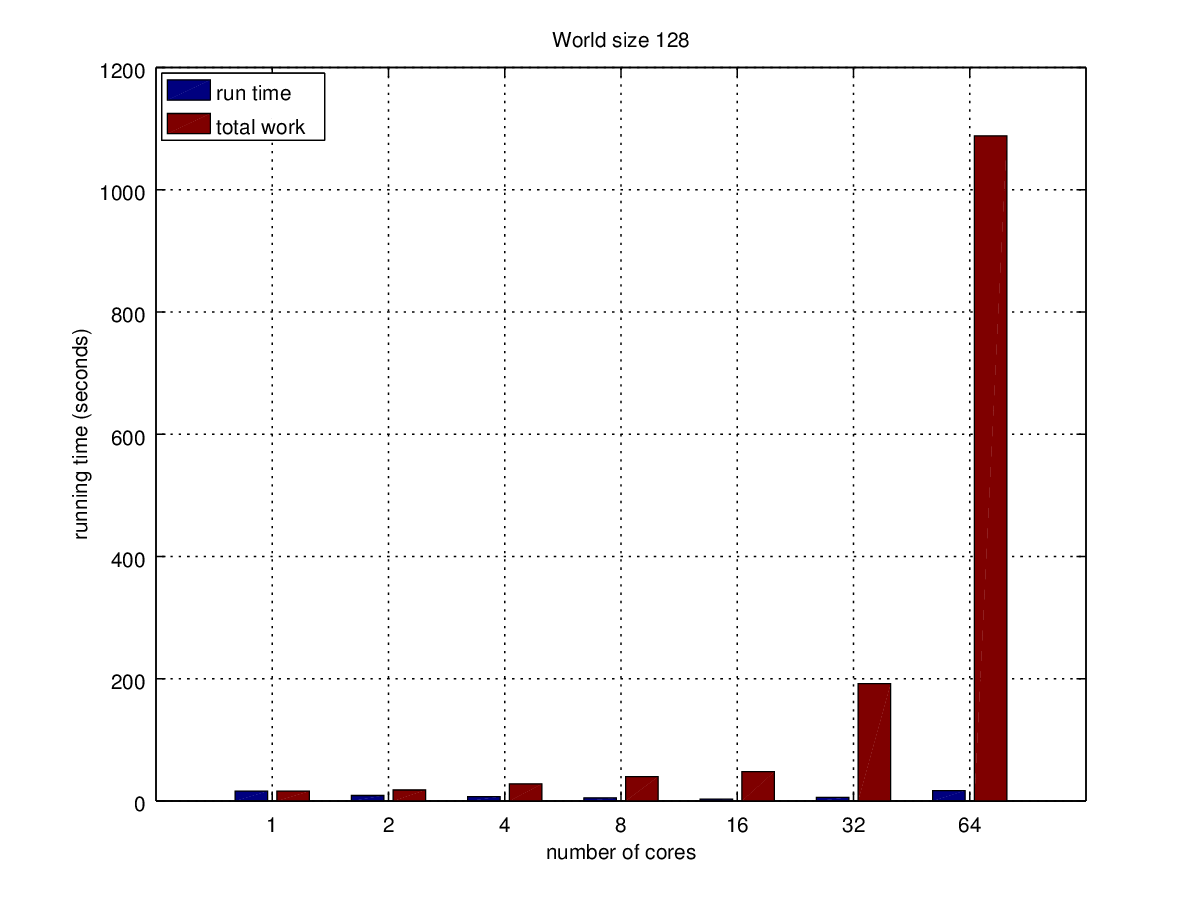
\includegraphics[width=\textwidth]{scaling-128}
    \caption{Scaling with world size $128 \times 128$}
\end{figure}

\begin{figure}
    \centering
    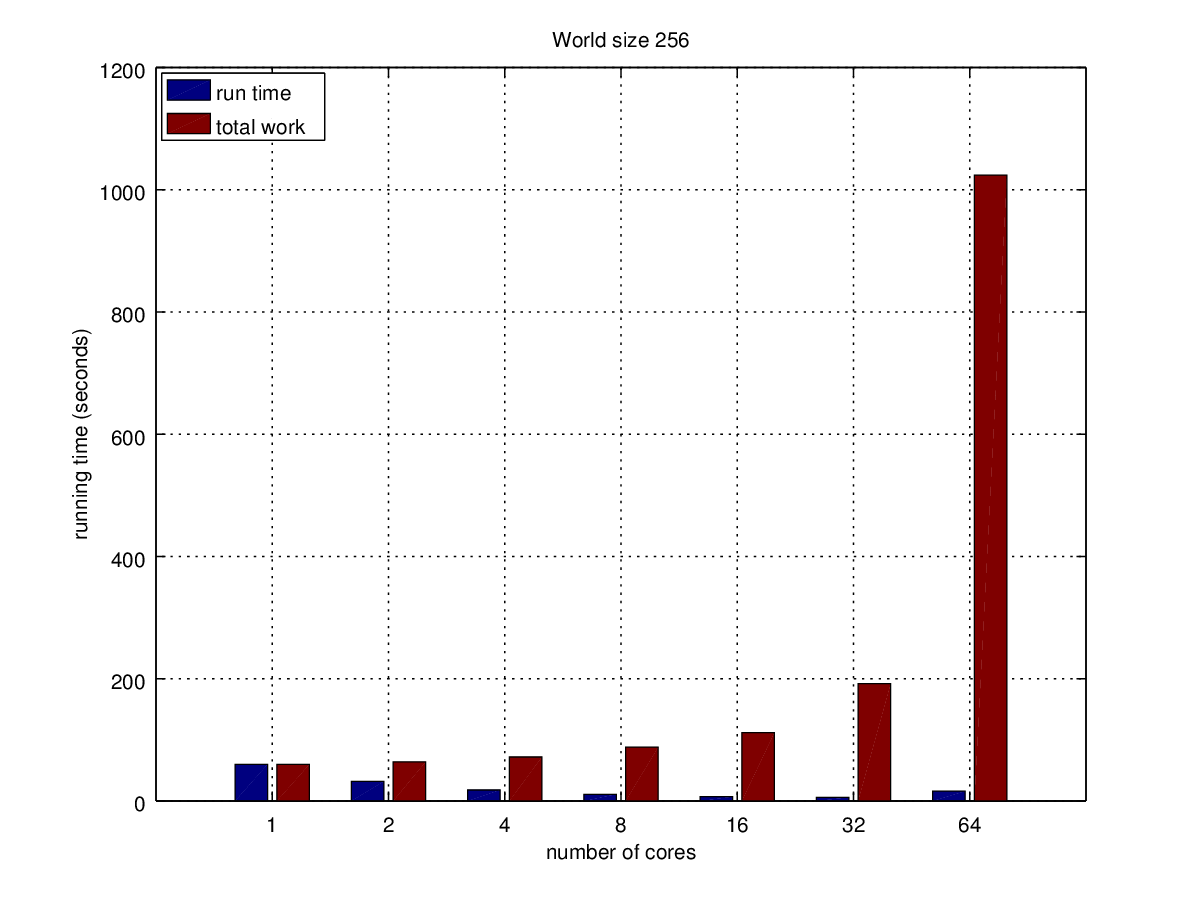
\includegraphics[width=\textwidth]{scaling-256}
    \caption{Scaling with world size $256 \times 256$}
\end{figure}

\begin{figure}
    \centering
    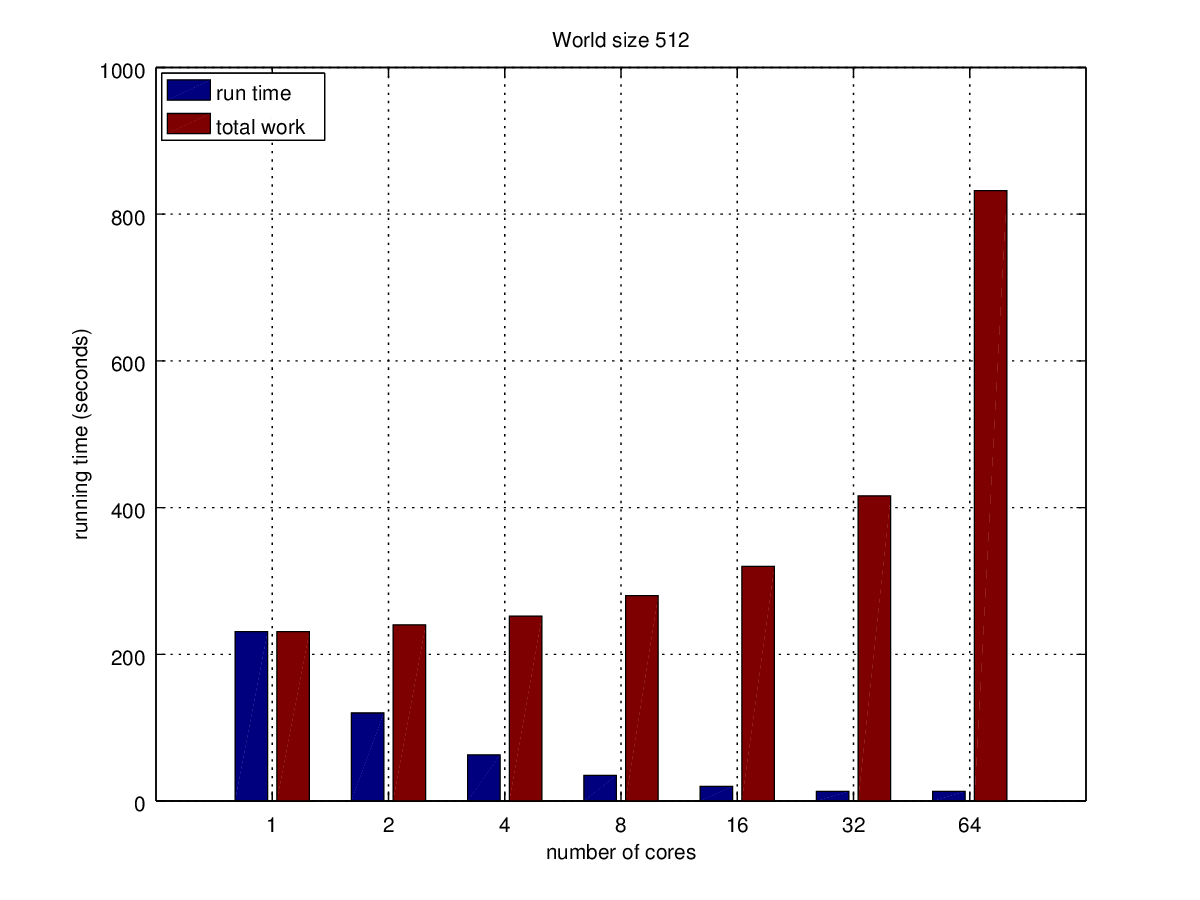
\includegraphics[width=\textwidth]{scaling-512}
    \caption{Scaling with world size $512 \times 512$}
\end{figure}

\begin{figure}
    \centering
    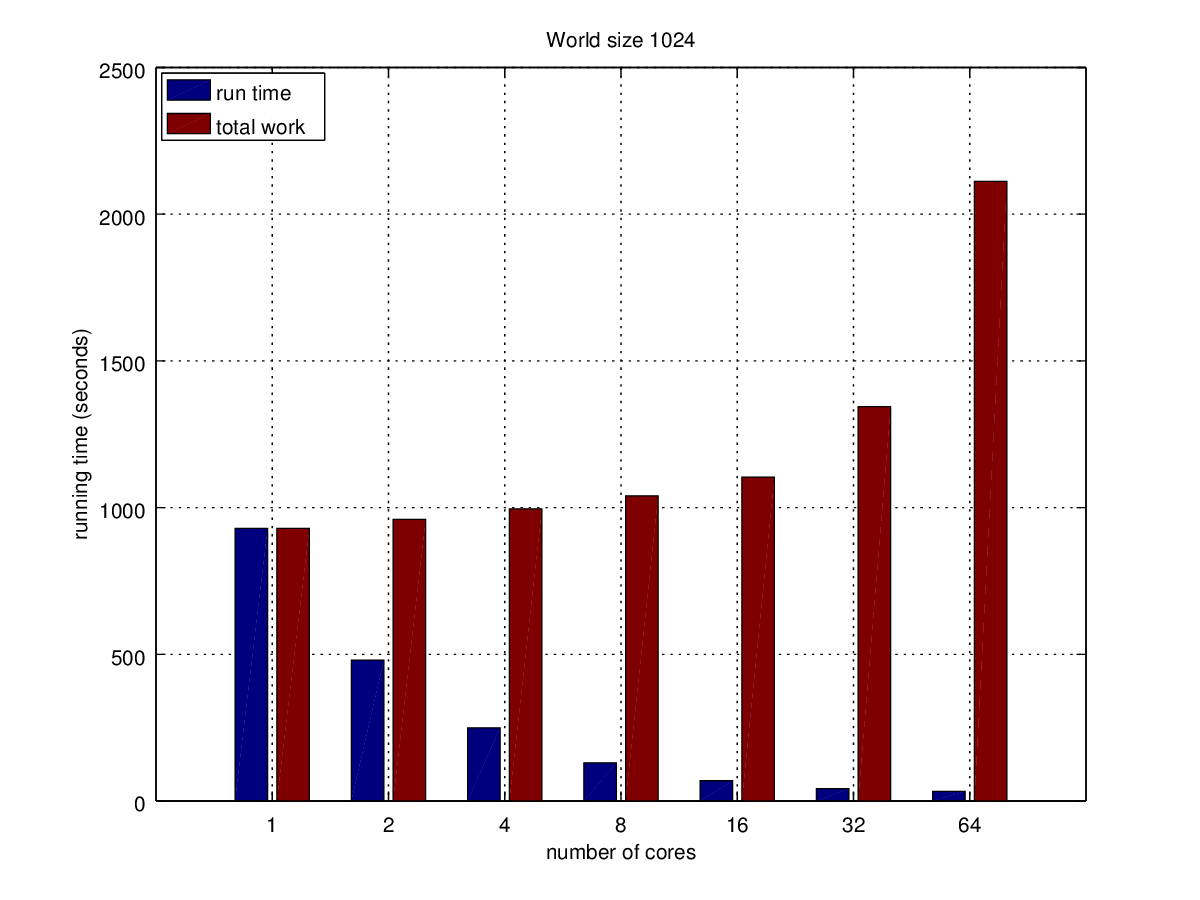
\includegraphics[width=\textwidth]{scaling-1024}
    \caption{Scaling with world size $1024 \times 1024$}
\end{figure}

\begin{figure}
    \centering
    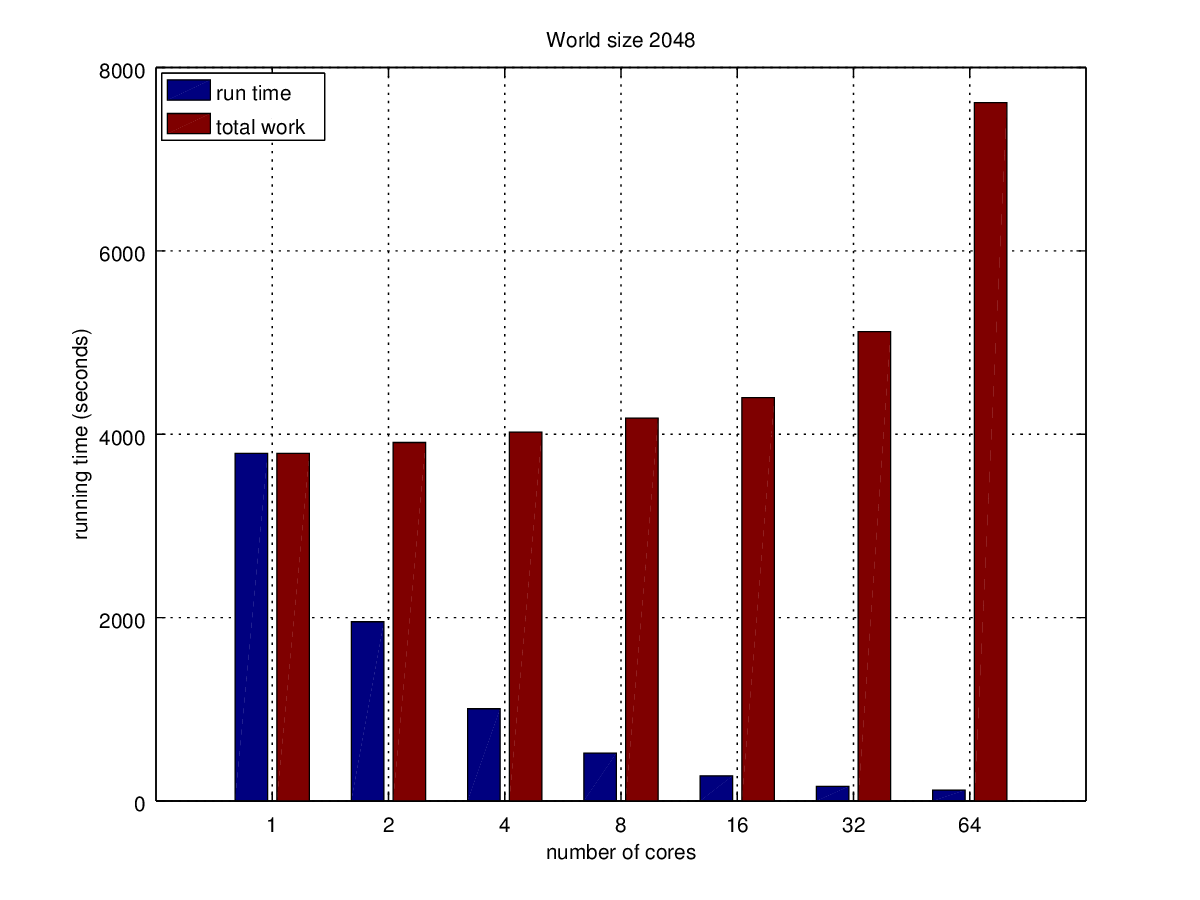
\includegraphics[width=\textwidth]{scaling-2048}
    \caption{Scaling with world size $2048 \times 2048$}
\end{figure}

\begin{figure}
    \centering
    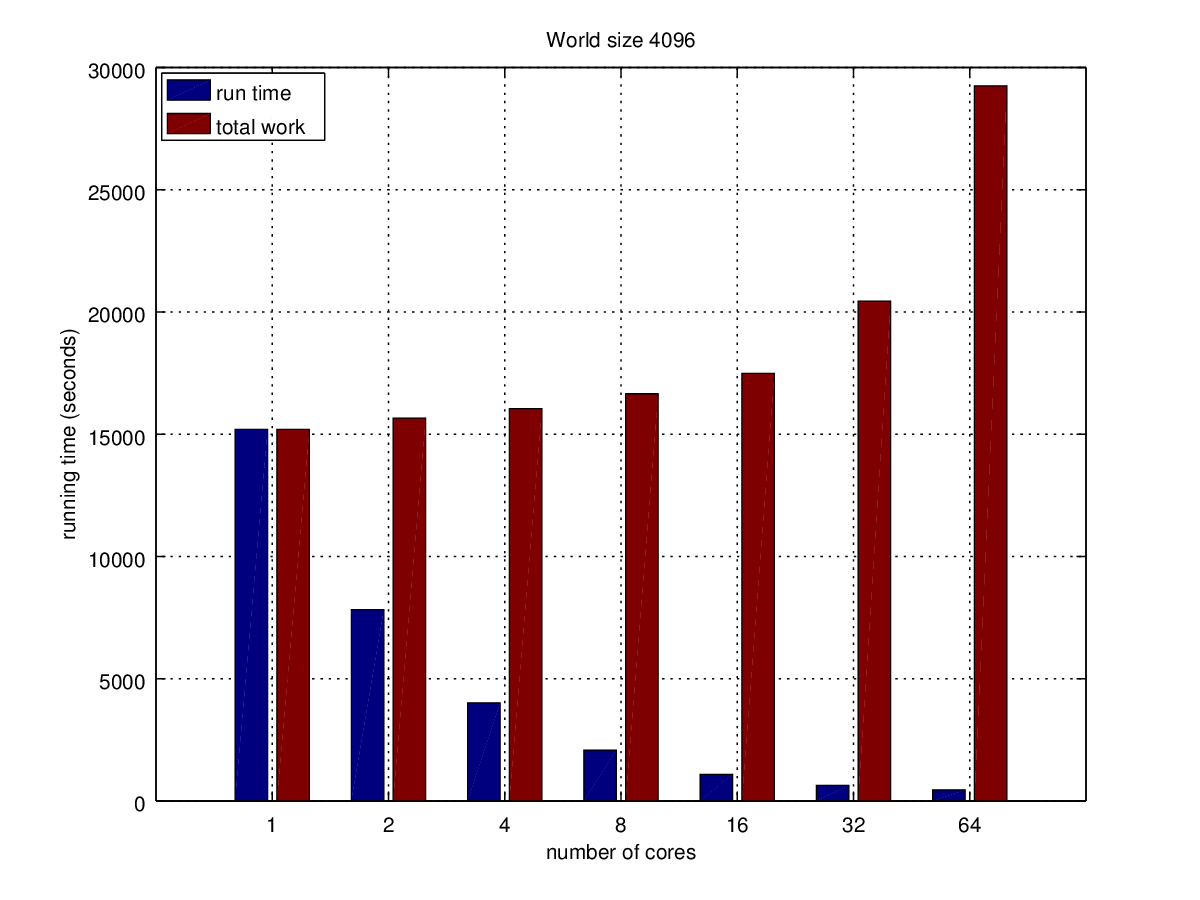
\includegraphics[width=\textwidth]{scaling-4096}
    \caption{Scaling with world size $4096 \times 4096$}
\end{figure}

\begin{figure}
    \centering
    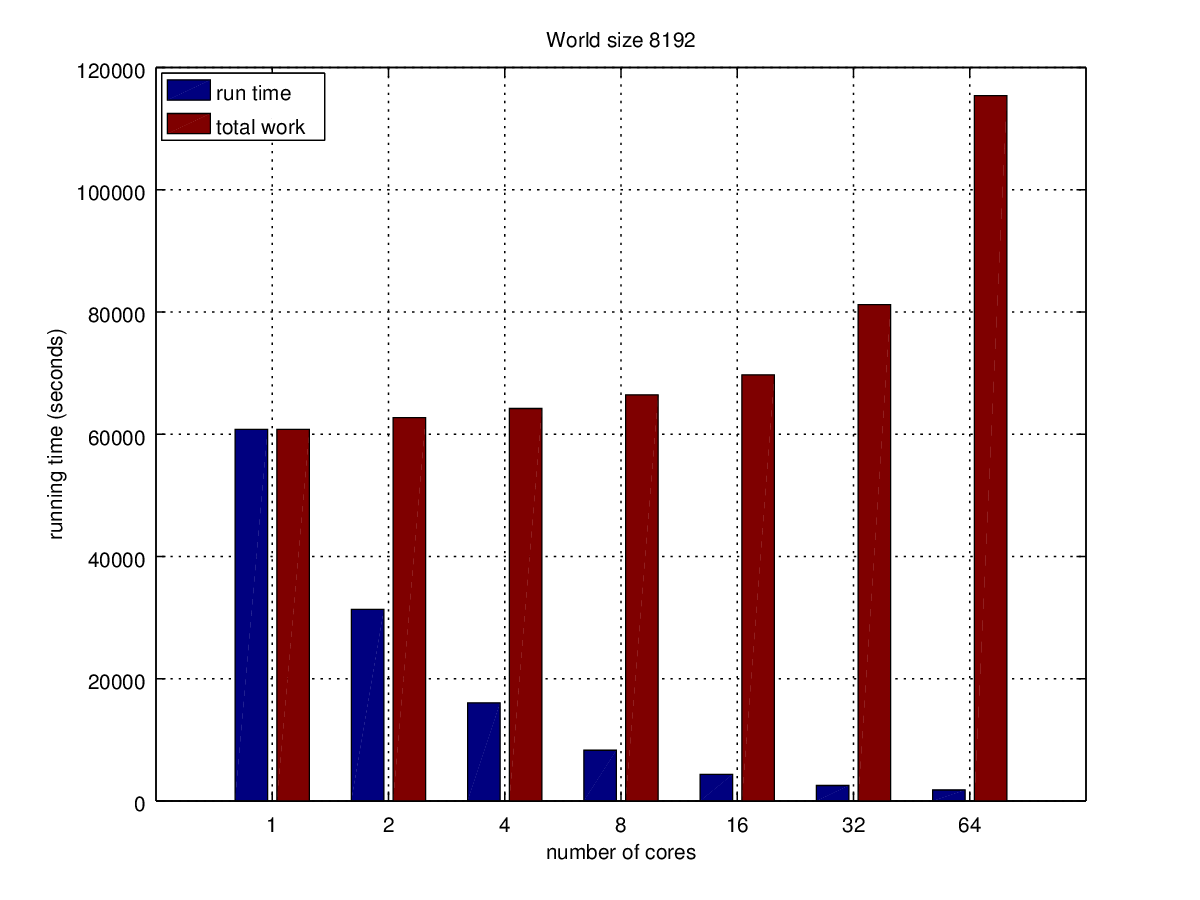
\includegraphics[width=\textwidth]{scaling-8192}
    \caption{Scaling with world size $8192 \times 8192$}
\end{figure}

\begin{figure}
    \centering
    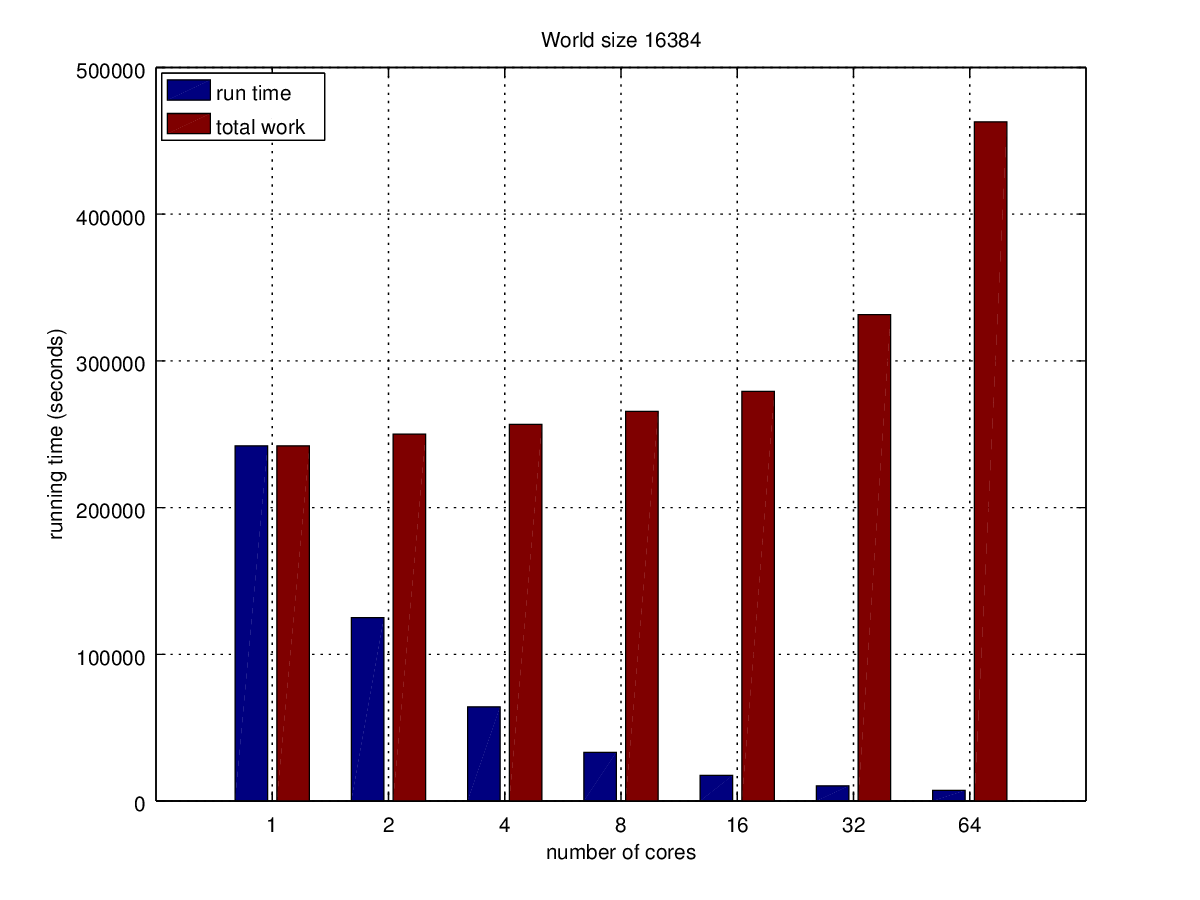
\includegraphics[width=\textwidth]{scaling-16384}
    \caption{Scaling with world size $16384 \times 16384$}
\end{figure}


\subsubsection{Weak scaling on 1 node}

Weak scaling is concerned with how the run time varies with the number of threads for a constant problem size, which in this case is the number of cells to be processed.
We evaluated weak scaling by taking the square of the side length of the grid used in each simulation run and then dividing by the number of threads, hence associating each run time with the number of cells per thread for that run.
We then produced a plot with the cells per thread on the x axis, and the run-time on the y axis; each simulation run is represented by a single point on the plot.
At first we tried using linear scales, but we found that a log-log scale best illustrates the results, shown in figure~\ref{weakscaling}.
This makes sense upon considering that the world sizes that we used for the test runs were exponentially increasing, from 128, 256, 512 and so on, and a similar exponential growth in the number of threads; 1, 2, 4, 8 up to 64.
It also makes sense that such exponential growth in the size of the world would also produce exponentially increasing run-times, since in the ideal case the run-time is directly proportional to the number of threads.

From the plot, we can see that when different simulation runs had the same number of cells per thread their run-times were also very close together.
Over a range of cells per thread, we can see a strong linear relationship with the run-time provided there is at least $2^{13}$ cells to a thread.

\begin{figure}
    \centering
    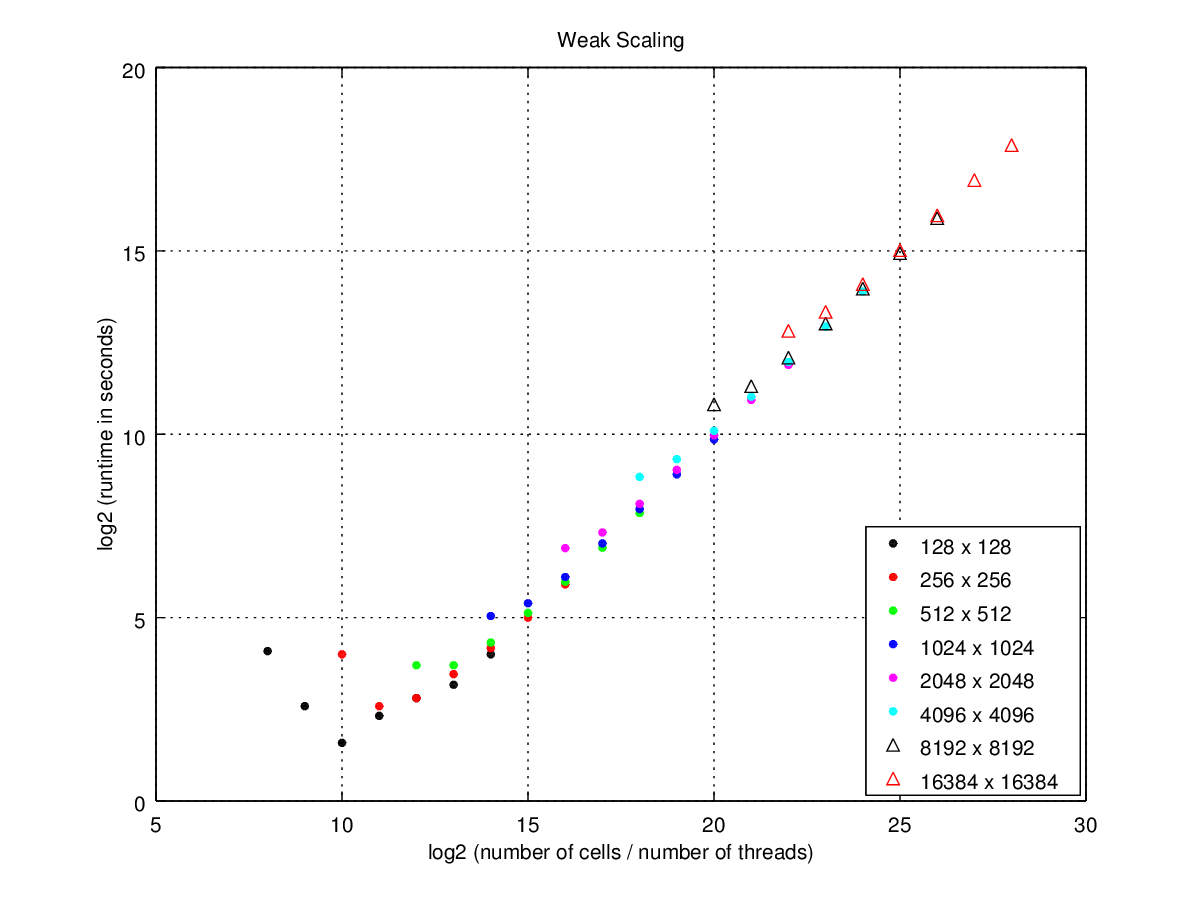
\includegraphics[width=\textwidth]{weak-scaling}
    \caption{Weak scaling on 1 node}
	\label{weakscaling}
\end{figure}

\subsubsection{Scaling with MPI}

We used a similar technique to measure the scaling when MPI was used for communication between multiple nodes of the Avoca cluster.
Instead of just the number of threads on one single node, we are now interested in the growth in the run-time as we run the simulation accross more nodes.
The following plots show strong scaling as more nodes were used, with an additional bar for the total amount of time that the simulation spent idle, waiting for network messages to be sent between nodes.

\begin{figure}
    \centering
    \includegraphics[width=\textwidth]{mpi-scaling-2048}
    \caption{Scaling using various number of nodes with world size $2048 \times 2048$}
\end{figure}

\begin{figure}
    \centering
    \includegraphics[width=\textwidth]{mpi-scaling-4096}
    \caption{Scaling using various number of nodes with world size $4096 \times 4096$}
\end{figure}

\begin{figure}
    \centering
    \includegraphics[width=\textwidth]{mpi-scaling-8192}
    \caption{Scaling using various number of nodes with world size $8192 \times 8192$}
\end{figure}

\begin{figure}
    \centering
    \includegraphics[width=\textwidth]{mpi-scaling-16384}
    \caption{Scaling using various number of nodes with world size $16384 \times 16384$}
\end{figure}


\begin{figure}
    \centering
    \includegraphics[width=\textwidth]{mpi-weak-scaling}
    \caption{Weak scaling using MPI}
\end{figure}

\subsection{Planet}

After performing all tests which were described in the previous section, we ran a simulation of zombie infection on a small toroidal planet.

\subsubsection{Size}

We originally wanted to simulate a world of size $32768 \times 16384$, equivalent to the surface of planet Earth, but unfortunately this was not possible because our implementation of 3D torus visualisation limits the texture size to no larger than $8192 \times 8192$.
The necessary modification to combine several textures inside OpenGL shaders would be too big burden.
Instead, we simulated a world of size $8192 \times 4096$; the disproportion of sizes is intentional as we definitely want to render cells as squares or close to squares.
They will be distorted mostly around equators: shrunken near inner equator and widened near the outside one.
In our case the ratio between major and minor radii is $ 2 : 1$.

\begin{figure*}[ht]
    \centering
    \begin{tabu} {| X[0.8,c,p] | X[0.9,c,p] || X[1,c,p] | X[1,c,p] | X[1,c,p] | X[0.9,c,p] |}
        \rowfont{\bfseries}
        \hline
        Nodes &
        Threads &
        Run-time (seconds) &
        Input border waiting (ms/iter) &
        Output border waiting (ms/iter) &
        Total MPI waiting (\%) \\
        \hline
        \hline
        64 & 32 & 30.665 & 3.531 & 2.104 & 18.376 \\
        \hline
        64 & 64 & 31.529 & 3.770 & 2.135 & 18.729 \\
        \hline
        128 & 32 & 17.793 & 2.763 & 1.757 & 25.402 \\
        \hline
        128 & 64 & 19.726 & 3.134 & 2.007 & 26.059 \\
        \hline
        256 & 32 & 13.539 & 2.437 & 1.552 & 29.467 \\
        \hline
        256 & 64 & 26.549 & 3.664 & 2.068 & 21.590 \\
        \hline
    \end{tabu}
    \caption{Scaling depending on number of threads}
\end{figure*}

Before we ran the simulation, we tried how well our application scale for this particular size.
The best option was to run the simulation with 32 threads on 128 nodes, with the world broken into segments of size $512 \times 512$.

\subsubsection{Tool-chain}

During the development of our simulation we created many scripts of various complexity.
Here we will describe their purposes and how they fit into the scheme of processing the results.
Their order correspond with their age and importance in data processing.

\begin{itemize}
\item apocalypse -- C program. Takes 4 numbers as arguments: width, height, number of zombies, number of iterations.
    It also has many features which are controllable by compile-time macros:
    \begin{itemize}
    \item \verb|NIMAGES| -- disables images generation
    \item \verb|NPOPULATION| -- disables output of population statistics
    \item \verb|NDETAILED_STATS| -- disables output of detailed population statistics
    \item \verb|NCUMULATIVE_STATS| -- disables cumulative (summed) statistics
    \item \verb|OUTPUT_EVERY=N| -- creates images and prints statistics every N steps
    \item \verb|IMAGES_EVERY=N| -- the same for images only
    \item \verb|POPULATION_EVERY=N| -- the same for population statistics only
    \item \verb|USE_MPI| -- enables usage of MPI (necessary for running on several nodes)
    \item \verb|REDIRECT| -- forces redirection of stdout and stderr when running on one node 
    \end{itemize}
\item visualise -- C program. Takes a step image produced by apocalypse and creates a png representing the current mesh situation.
    Different entities are rendered in different colours; each one is a single pixel.
\item plot.py -- Python script. Reads population statistics from standard input and either shows or produces an image of population sizes in time.
\item demographics -- C program. Takes a step image and produces a file containing aggregated information about ages of all entities.
\item histogram.py -- Python script. Reads aggregated demographics information from standard input and either shows or produces and image of histogram of ages distribution.
\item globalise -- C program. Takes either several population statistics files or step images (all of the same time-step) and combines them into a single file.
    The result emulates the situation as if the the simulation was running on a single node.
\item torus -- C++ program. Takes a png image representing texture of a torus and shows a 3D visualisation of toroidal planet.
    The program can be either interactive allowing simple movement and ad-hoc image creation or forced to produce a single image and exit.
\item process\_planet.py -- Python script. Takes all error outputs from apocalypse and calculates statistics about running and waiting times.
\item planet\_task.py -- Python script. Creates an sbatch script and runs sbatch. 
\end{itemize}

The process of running apocalypse, transferring and processing results is shown on the diagram.

\begin{figure*}[pht]
    \centering
    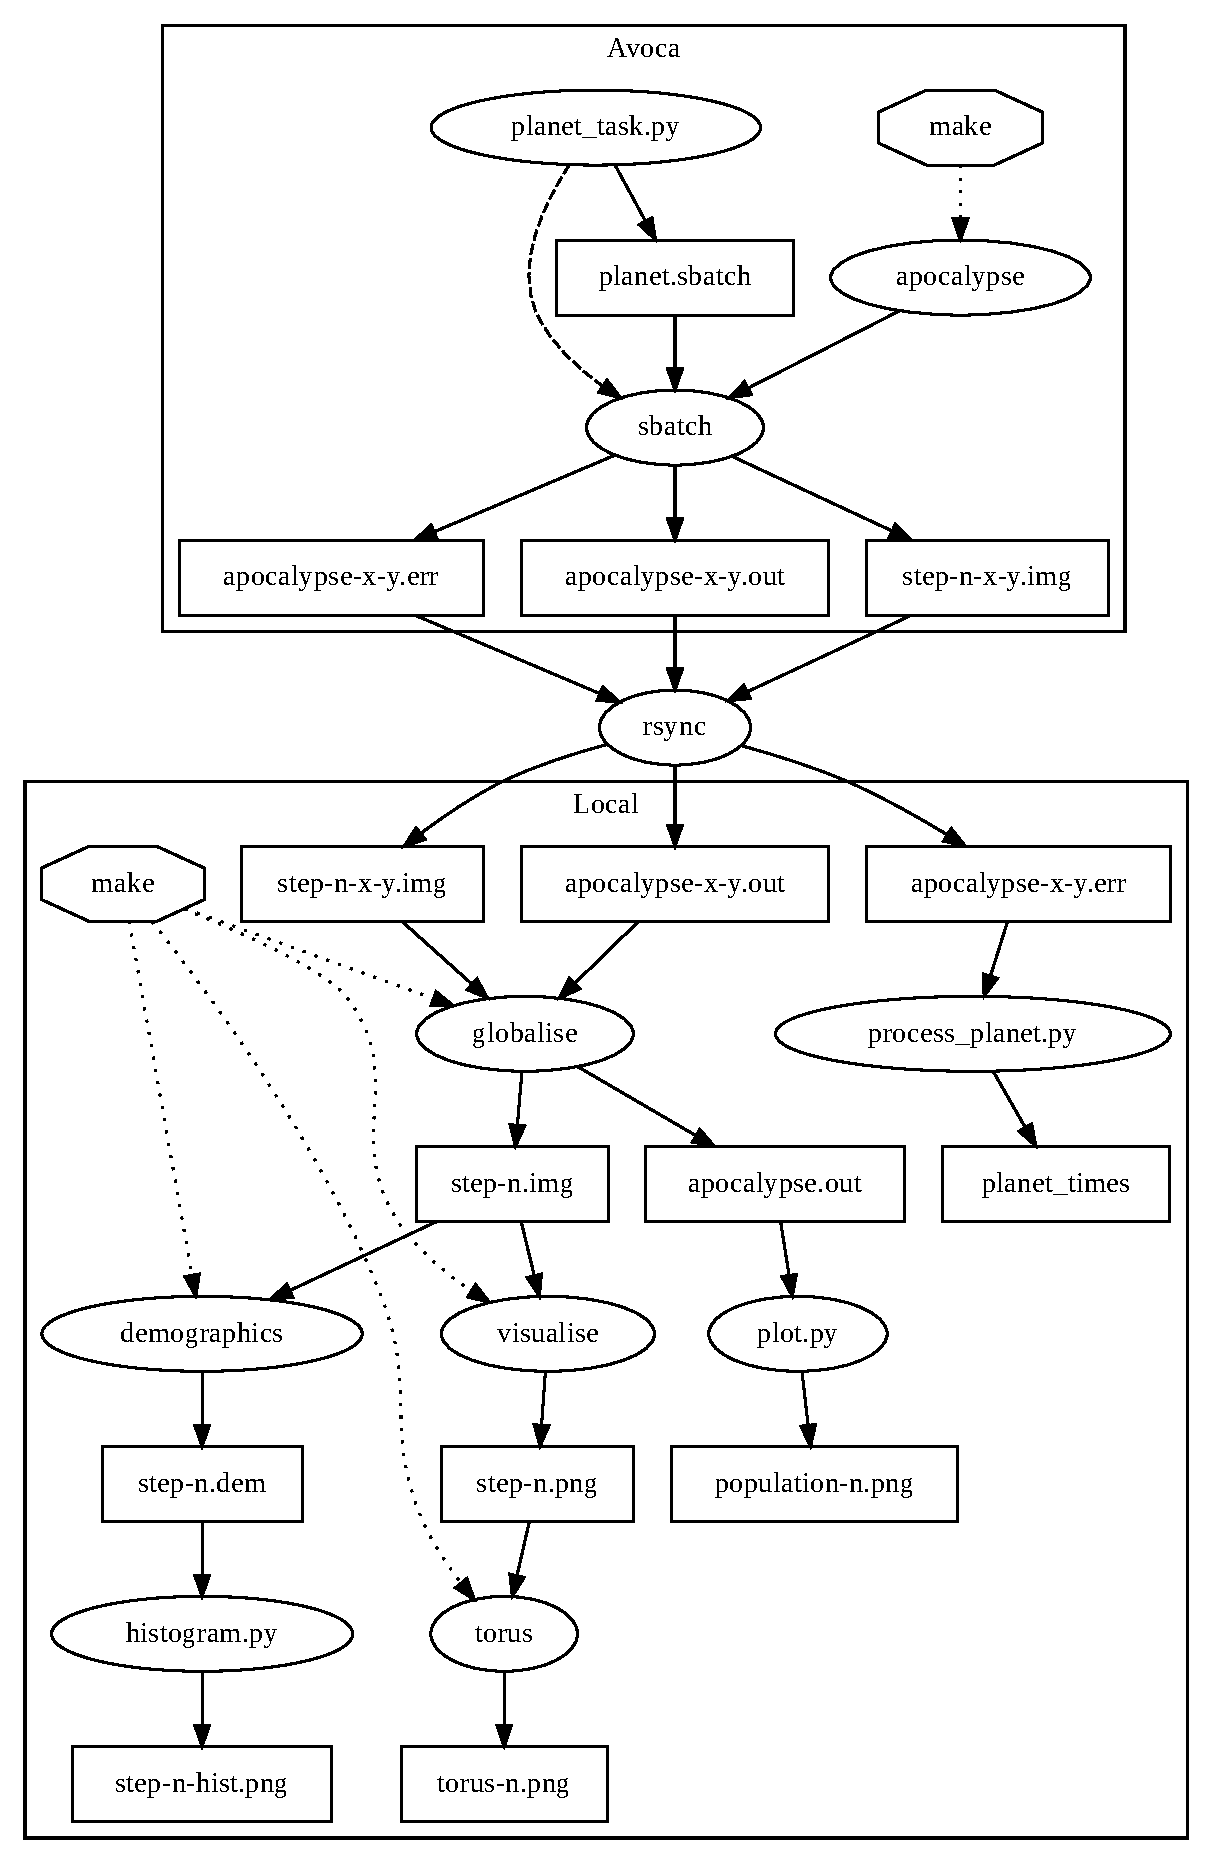
\includegraphics[width=\textwidth]{toolchain}
    \caption{Toolchain with intermediate files}
\end{figure*}

\subsubsection{Run-time and data amount}

We ran the simulation for 2~hours of computation time on 128~nodes.
During this period, 588,745~days (1613~years) were simulated.
To preserve disk-space and also make the computation not I/O speed dependent, we chose to save the world images every 365~days.

As the world is split into 128~parts, each of them producing independent files, we obtained 206,592~files of average size 150~KB and total size 30~GB just for world representation.
We also obtained $128 + 128$ files capturing redirected standard output and standard error.
Err files are of size 57~MB each and output files are 209~MB each; this is about 34~GB in total.
Fortunately, all these files are very simple and easy to compress.

The globalised world representations are of size 16~MB and resulting png images (of size $8192\times 4096$ pixels) are 2.8~MB each.
The globalised world statistics (standard output) are in a single file of size 218~MB.

The time spent by waiting for MPI sends and receives was 2.252 and 1.961~ms per iteration, which means that the program waited for MPI for 34.44\% of total time.

\subsubsection{Visualisation in time}

Populations during the simulation of a whole planet are more stable than in the case of world of size 500 by 500; this can be seen on the populations figure.
The number of people decreases linearly as increases the number of zombies.
As soon as the zombies fill whole planet, the population sizes no longer change.
The cause is that the borders are no longer significant for zombie infection spreading.
If we increased the probability of infection, we suppose that the populations would still be stable, though we haven't tried that.

In the figures of the toroidal planet, there is clearly visible a consequence of the bug discussed later in the issues section (borders of world parts have less population density).

\begin{figure*}[ht]
    \centering
    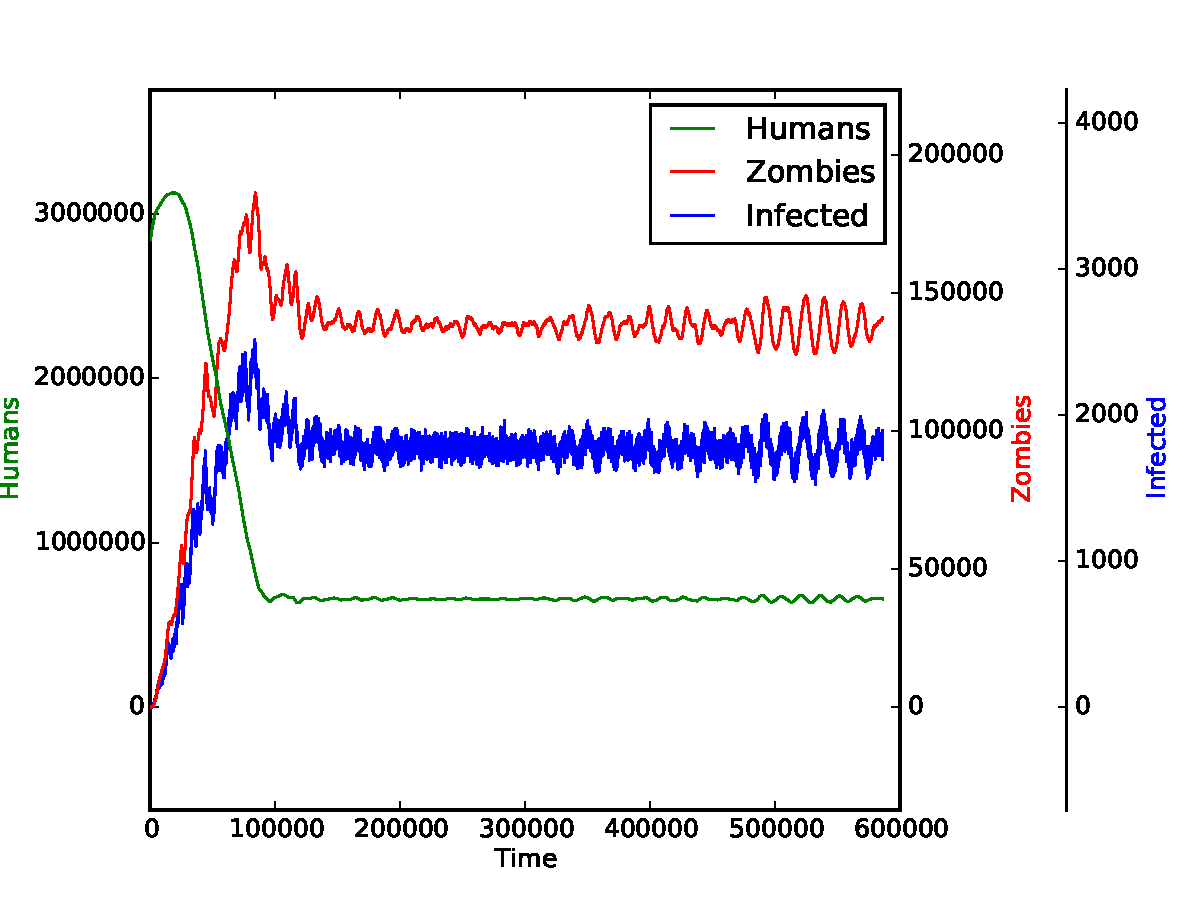
\includegraphics[width=\textwidth]{torus/planet.pdf}
    \caption{Populations sizes on the planet withing 1613 years}
\end{figure*}

\begin{figure*}[pht]
    \centering
    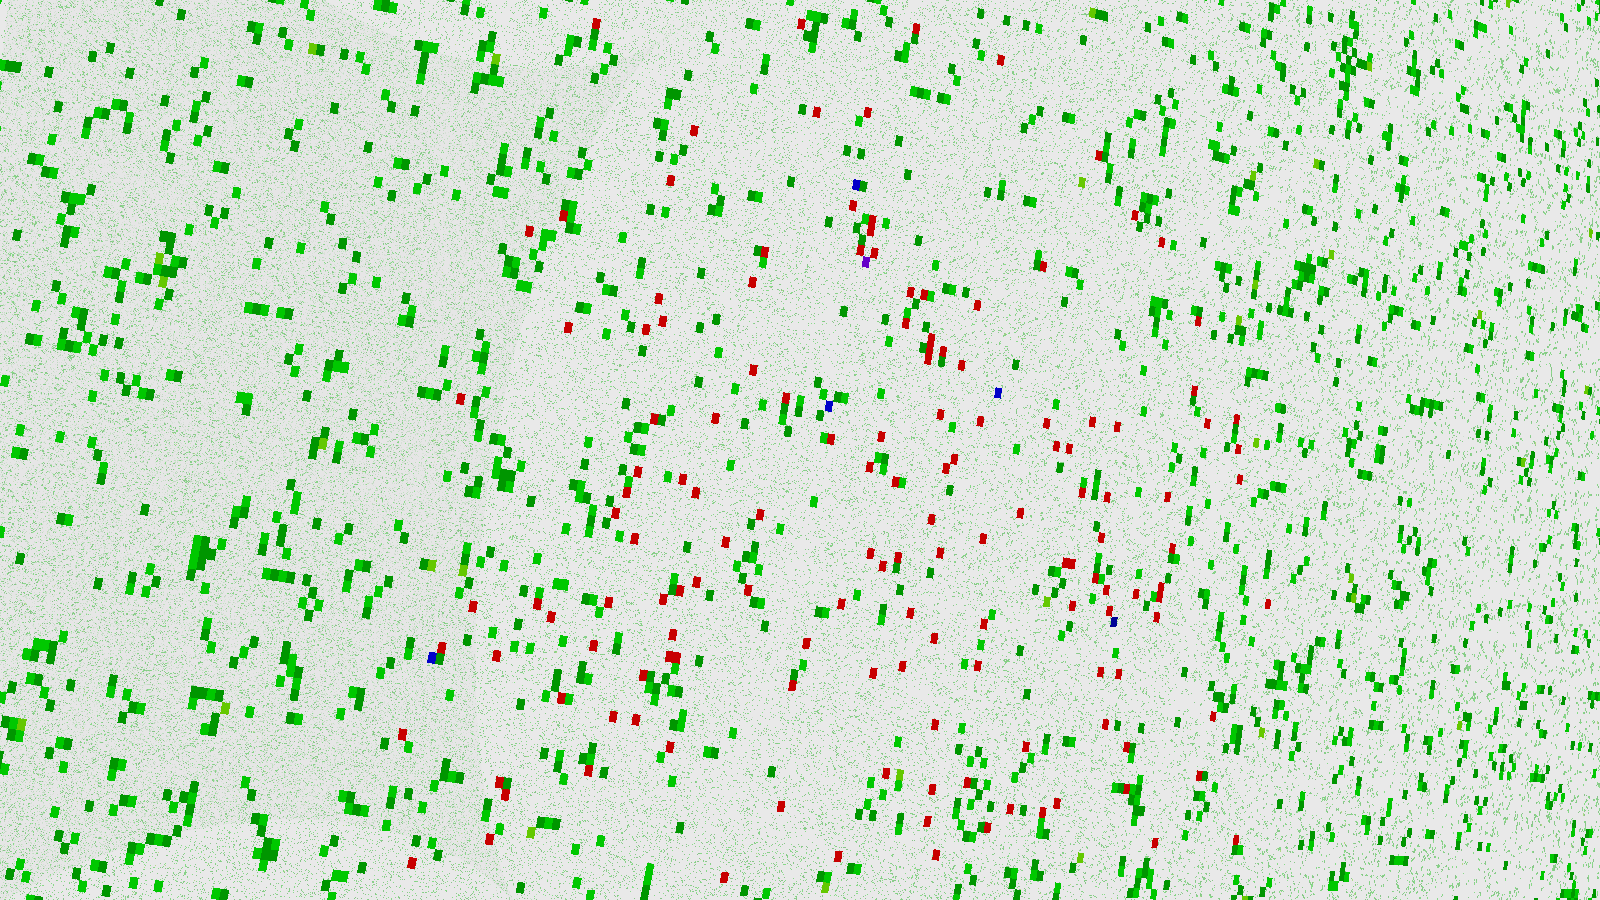
\includegraphics[width=\textwidth]{torus/step-002190-torus.png}
    \caption{Planet after 6 years; one of two initial zombie clusters}
    \includegraphics[width=\textwidth]{step-002190.pdf}
    \caption{Demographics after 6 years}
\end{figure*}

\begin{figure*}[pht]
    \centering
    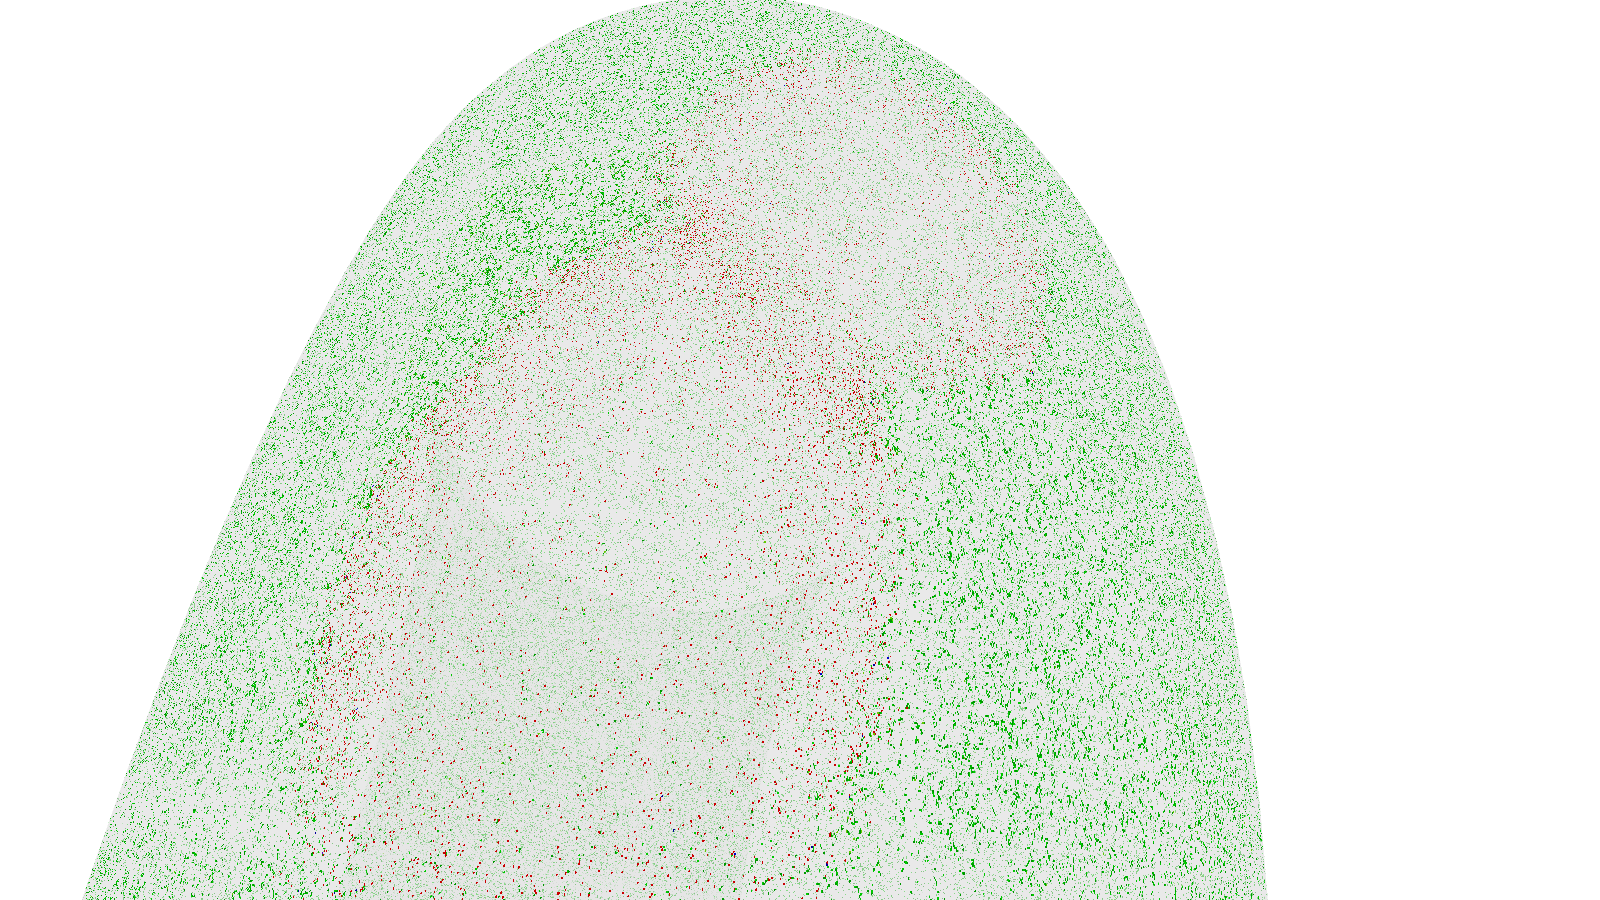
\includegraphics[width=\textwidth]{torus/step-006935-torus.png}
    \caption{Planet after 19 years; clusters are starting to merge}
    \includegraphics[width=\textwidth]{step-006935.pdf}
    \caption{Demographics after 19 years}
\end{figure*}

\begin{figure*}[pht]
    \centering
    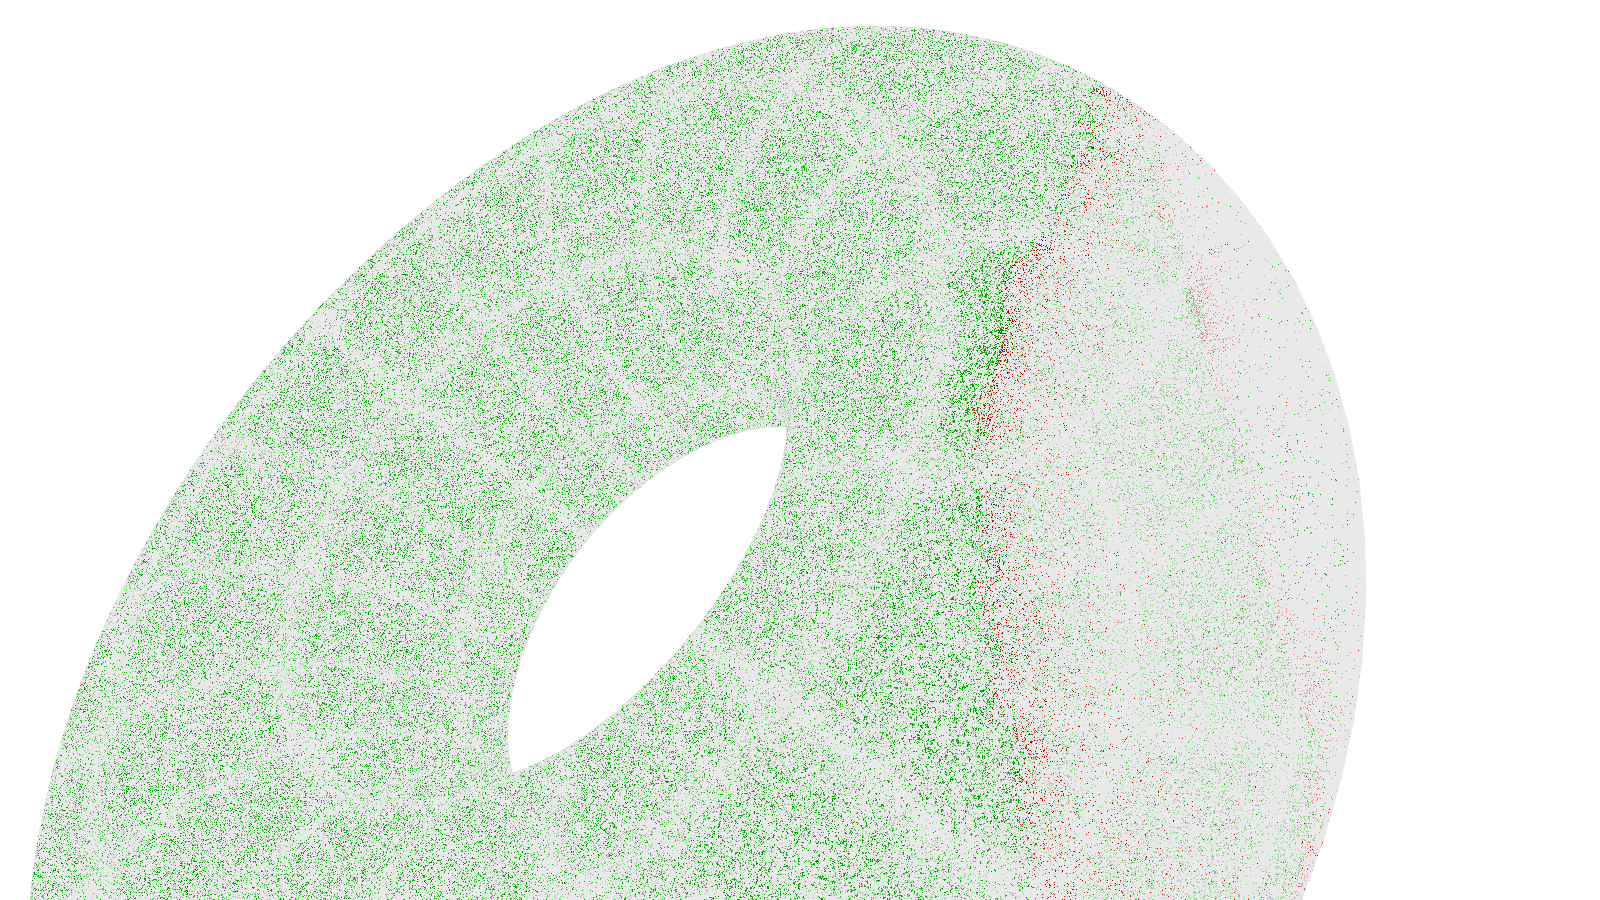
\includegraphics[width=\textwidth]{torus/step-016790-torus.png}
    \caption{Planet after 46 years; one side is occupied by zombies}
    \includegraphics[width=\textwidth]{step-016790.pdf}
    \caption{Demographics after 46 years}
\end{figure*}

\begin{figure*}[pht]
    \centering
    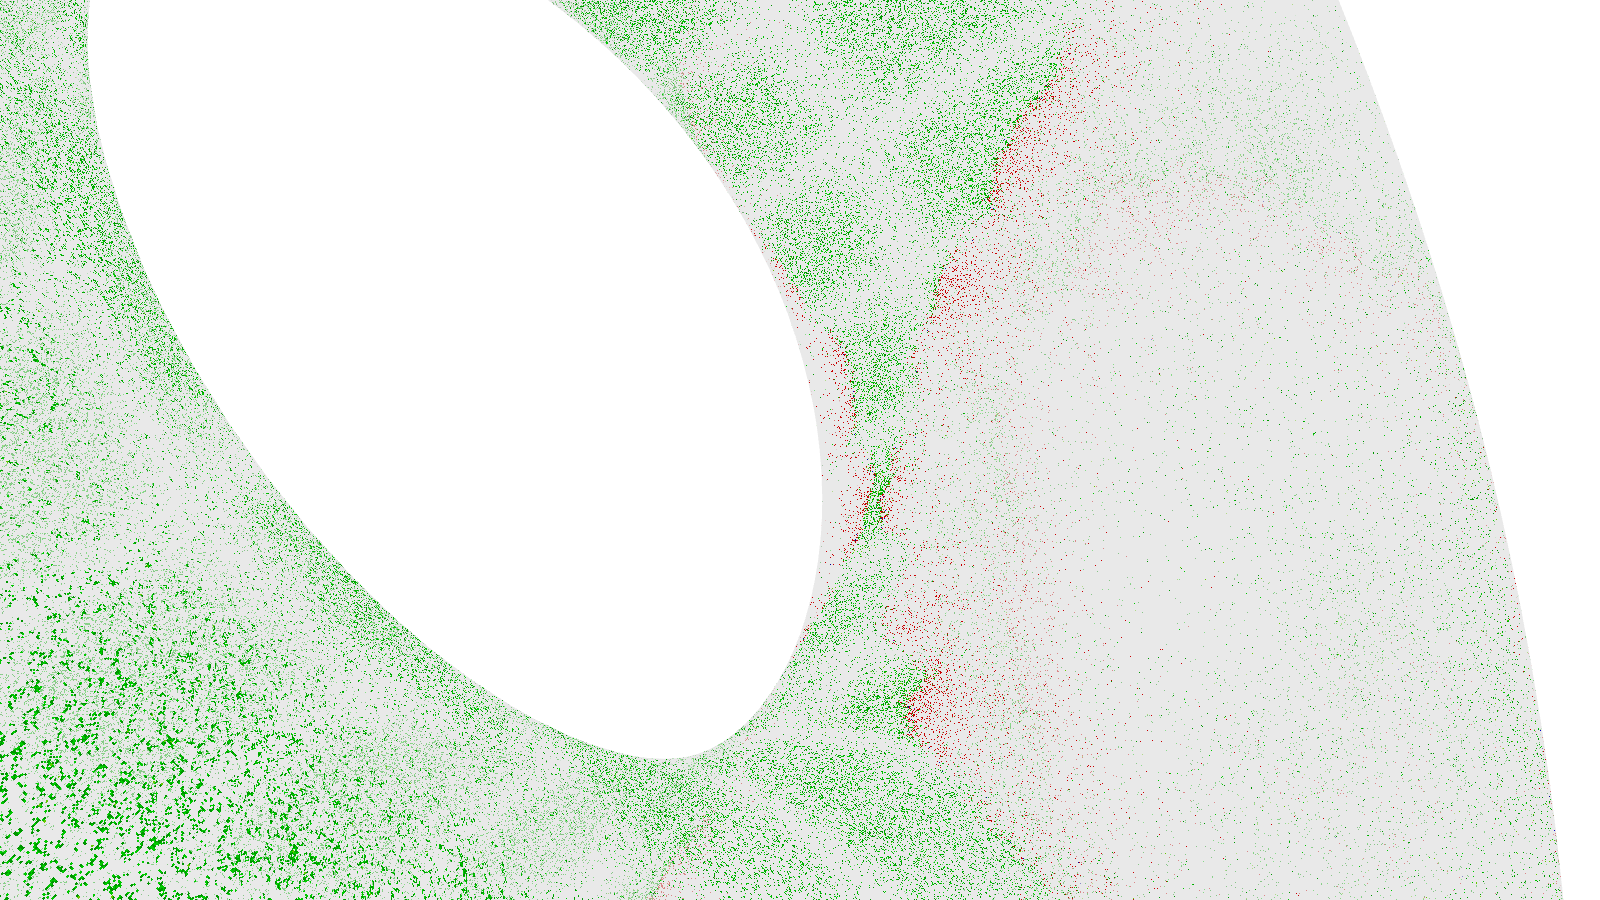
\includegraphics[width=\textwidth]{torus/step-042340-torus.png}
    \caption{Planet after 116 years; connecting around the toroidal body}
    \includegraphics[width=\textwidth]{step-042340.pdf}
    \caption{Demographics after 116 years}
\end{figure*}

\begin{figure*}[pht]
    \centering
    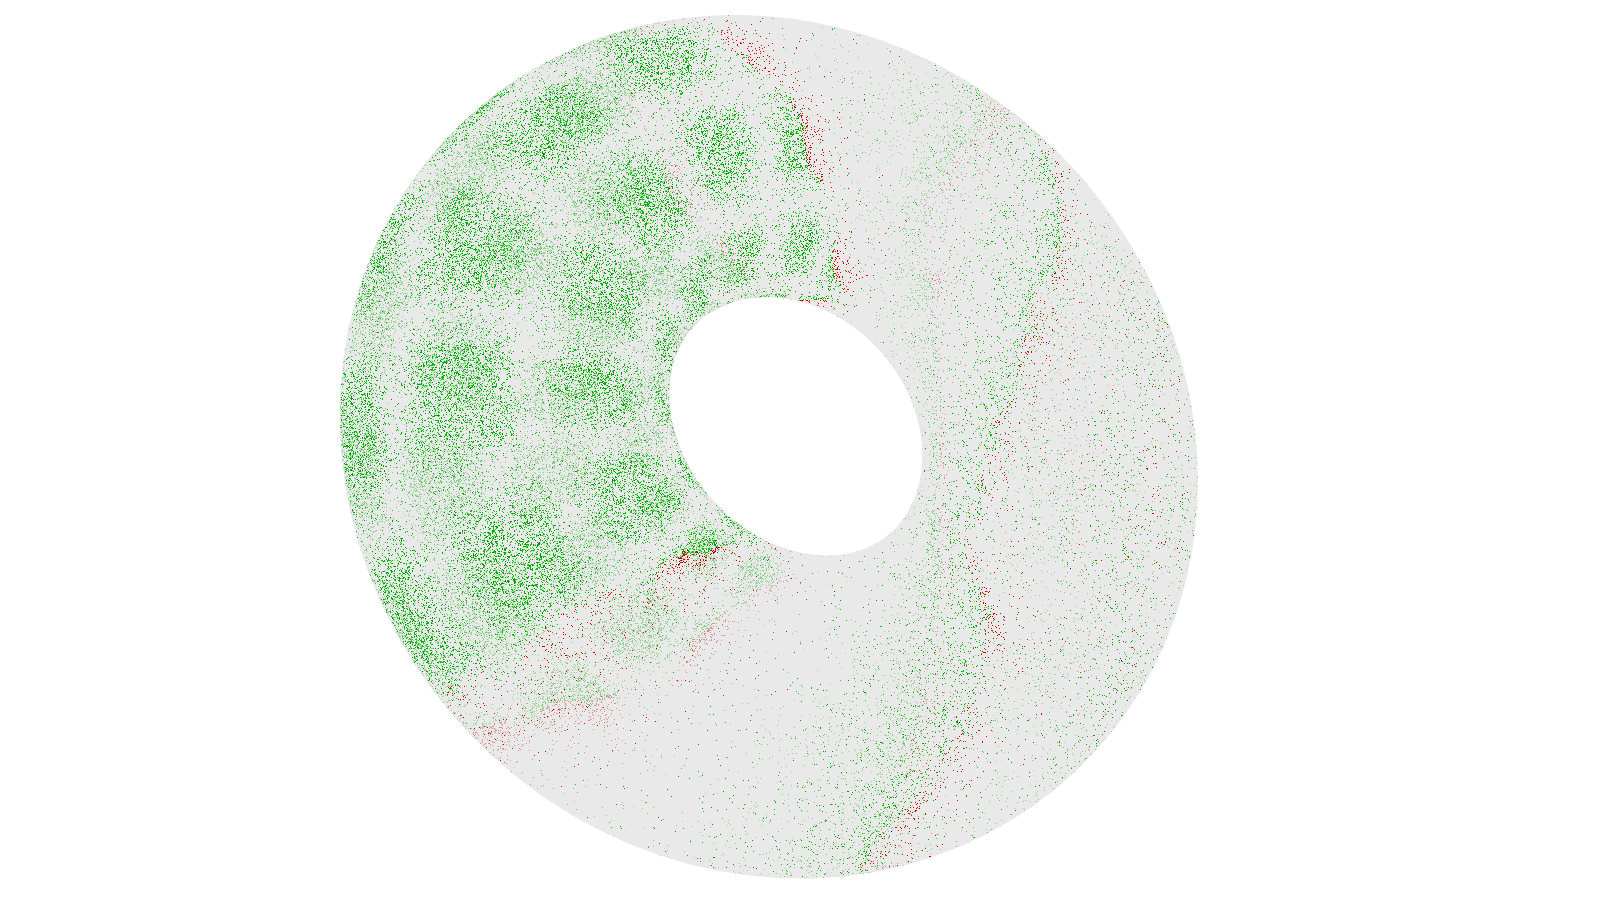
\includegraphics[width=\textwidth]{torus/step-059130-torus.png}
    \caption{Planet after 162 years; zombies control most of the planet; a second wave of humans and zombies is forming}
    \includegraphics[width=\textwidth]{step-059130.pdf}
    \caption{Demographics after 162 years}
\end{figure*}

\begin{figure*}[pht]
    \centering
    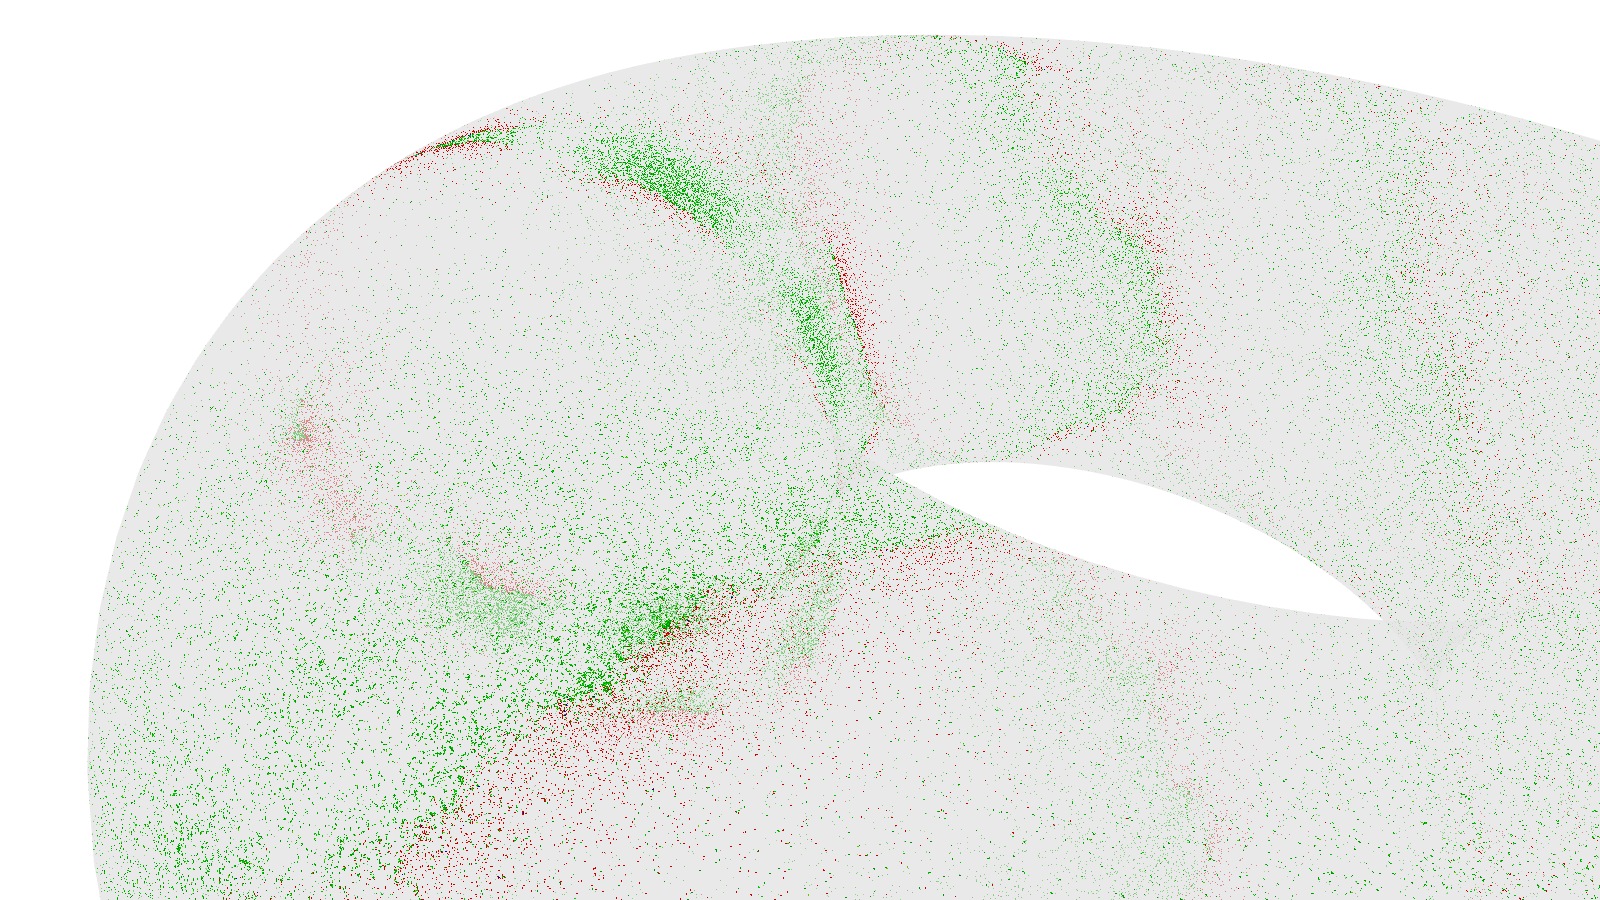
\includegraphics[width=\textwidth]{torus/step-084315-torus.png}
    \caption{Planet after 231 years; a small strip of people is left; the second and the third wave is noticeable}
    \includegraphics[width=\textwidth]{step-084315.pdf}
    \caption{Demographics after 231 years}
\end{figure*}

\begin{figure*}[pht]
    \centering
    \includegraphics[width=\textwidth]{torus/step-091615-torus.png}
    \caption{Planet after 251 years; the last people who were unaffected by zombies}
    \includegraphics[width=\textwidth]{step-091615.pdf}
    \caption{Demographics after 251 years}
\end{figure*}

\begin{figure*}[pht]
    \centering
    \includegraphics[width=\textwidth]{torus/step-129575-torus.png}
    \caption{Planet after 355 years; stable situation has been reached}
    \includegraphics[width=\textwidth]{step-129575.pdf}
    \caption{Demographics after 355 years}
\end{figure*}

\begin{figure*}[pht]
    \centering
    \includegraphics[width=\textwidth]{torus/step-462820-torus.png}
    \caption{Planet after 1268 yearsl; still stable}
    \includegraphics[width=\textwidth]{step-462820.pdf}
    \caption{Demographics after 1268 years}
\end{figure*}

\begin{figure*}[pht]
    \centering
    \includegraphics[width=\textwidth]{torus/step-588745-torus.png}
    \caption{Planet after 1613 years; the last year of the simulation}
    \includegraphics[width=\textwidth]{step-588745.pdf}
    \caption{Demographics after 1613 years}
\end{figure*}

\section{Issues}

During the implementation we had to deal with many issues, here we mention some of them including one which is still present.

\subsection{Directed movement}

When implementing the simulation of entities movement on a 2D mesh, we chose to use two nested for loops (the outer went through columns, the inner through rows) copying entities from the input mesh to the outer one.
For each entity the optimal decision where to move was calculated (as discussed earlier) and then tested whether the destination cell is free.
Unfortunately the chosen direction of processing causes that the cells to the left and to the up are already processed and there exists a chance that those cells will contain an entity.
On the other hand, the cells to the right and to the down are unprocessed and therefore the conflict is less likely.
This slight inequality causes that the overall movement is targeted to right and down and clusters of entities appear the the world border.

These clusters proved to be important for zombies.
It is an ideal place where they can feast and keep their number high until the rest of the world regenerate.
They are also often places where the infection starts and spreads very quickly with creating a lot of zombies.

When the flaw was repaired (by randomising the processing directions), the zombies could not survive under the previously stable conditions.
No matter what changes we did to the model, the infection probability had to be lowered from original value 0.01 to 0.0075.
The new probability keeps the zombie population size of at least 100 individuals at all time.

\subsection{Too little iterations}

For the scaling part, we first tried to run only 10 iterations to preserve resources and make the task quicker.
This attempt lead first to a wrong conclusion that the scaling does not work due to slow CPU-memory access.
We disproved this result by comparing the run-times with older versions of our program.
We noticed an unreasonable slow-down.

The cause was:
\begin{itemize}
\item either too intensive I/O -- we saved the world to files after every step,
\item or slow initialisation of OpenMP and caches.
\end{itemize}

We solved this issue by running the simulation for 1000 steps and saving the world each 100 steps.

\subsection{Collisions at the border}

All processes except for movement depend only on the input world.
Movement on the hand has to make sure that the place where the entity wants to move is free.
This is easy for the interior of the world, there we have information about movement in output world.
In the interior, when a collision is detected, an alternative is tried, and eventually the entity stays at it current cell.

However, the information is not available for border cells, there we just check collisions with input world.
At the border, when the world is dense enough, there are conflicts and the difference is noticeable.
Fortunately, the nature of our simulation guarantees that the density will lower over time to a value when we expect negligible number of collisions.

Dealing with this issue would either require locking (one world has to be processed before the other one).
The other option is simulation of one row/column in the border.
This would require to extend the border to 3 cells and synchronise random generators.
On the other hand, the transfer of entities from one world to the other one would not be necessary.

There is also an option to change the algorithm for movement for entities at the border to ignore cells which are in distance of two.
This leads to keeping the same border size but also to a minor intervention to algorithm which should be the same everywhere.

\section{Recommendations}

In the results section we have shown how crucial is to keep the right birth rate.
If it was underestimated, the human population drops very quickly and zombies die out as humans do a few decades later.
When it is overestimated, the simulation has the same result for zombies but is much more favourable for humans, which can eventually recover.
We found a function which describes the right conditions when both populations become stable and can coexist.

We therefore recommend and appeal the human population and its government to control their population size as we propose.
Especially in the beginning when the zombie population grows and the zombies spread over the Northern Territory, the people must be prepared for a big decline.
Although it will be hard at that time, they must seek each other and reproduce in order to make sure their population will survive.
Humans should not behave according to their instinct and hide until the zombies population has decreased; that would cause extinction of the zombies.



\begingroup
\raggedright

\bibliographystyle{IEEEtran}
\bibliography{references}
\endgroup

\end{document}

% vim: ft=tex ts=4 sw=4 et
